\documentclass[journal,compsoc,10pt,final]{IEEEtran}

\ifCLASSOPTIONcompsoc
\usepackage[caption=false,font=normalsize,labelfon
t=sf,textfont=sf]{subfig} \else
\usepackage[caption=false,font=footnotesize]{subfi
g} \fi
\usepackage{booktabs}
%\usepackage{subcaption}
\usepackage{listings}
\usepackage{graphicx}
\usepackage[ruled,linesnumbered]{algorithm2e}
\usepackage{url}
\usepackage{enumerate}
\usepackage{amsmath}
\usepackage{multirow}
\usepackage{makecell,rotating}
\usepackage{color, colortbl}

\def\BibTeX{{\rm B\kern-.05em{\sc i\kern-.025em b}\kern-.08em
    T\kern-.1667em\lower.7ex\hbox{E}\kern-.125emX}}

\newcommand\FIXME[1]{\textcolor{red}{FIX:}\textcolor{red}{#1}}
\newcommand\mypara[1]{\vspace{1.5mm}\noindent \textbf{#1}}


\begin{document}
\title{Optimizing Depthwise Separable Convolution Operations on GPUs}

\author{Gangzhao~Lu, Weizhe~Zhang,~\IEEEmembership{Senior Member, ~IEEE,} and~Zheng~Wang
\IEEEcompsocitemizethanks{
\IEEEcompsocthanksitem G. Lu and W. Zhang are with the School of Cyberspace Science at Harbin Institute of Technology, Harbin 150000, China.\protect\\
	E-mail:\{lugangzhao,wzzhang\}@hit.edu.cn
\IEEEcompsocthanksitem Z. Wang is with the School of Computing at University of Leeds, United Kingdom.\protect\\
	E-mail: z.wang5@leeds.ac.uk}}

\IEEEtitleabstractindextext{
\begin{abstract}
The depthwise separable convolution is commonly seen in convolutional neural networks (CNNs), and is widely used to reduce the
computation overhead of a standard 2D convolution. Existing implementations of depthwise separable convolutions target accelerating model
training with large batch size with a large number of samples to be processed at once. Such approaches are inadequate for
small-batch-sized model training and the typical scenario of model inferencing where the model takes in a few samples at once.
%
This paper aims to bridge the gap of optimizing depthwise separable convolutions by targeting the GPU architecture. We achieve this by
designing two novel algorithms to improve the column and row reuse of the convolution operation to reduce the number of memory operations
performed on the width and the height dimensions of the 2D convolution. Our approach employs a dynamic block size scheme to adaptively
distribute the computational data across GPU threads to improve the GPU utilization and to hide the memory access latency. We apply our
approach on two GPU platforms: an NVIDIA RTX 2080Ti GPU and an embedded NVIDIA Jetson AGX Xavier GPU. We compared our approach against
cuDNN that is heavily tuned for the NVIDIA GPU architecture. Experimental results show that our approach delivers over $2\times$ (up to
$3\times$) performance improvement over cuDNN. We show that our approach reduces the end-to-end training and inference time of MobileNet
when the using a moderate batch size by 14.4\% and 9.7\% on average, respectively.


%In recent years, depthwise separable convolutions have been used in many convolutional neural networks (CNNs) to reduce the computational cost of standard 2D convolutions.
%Depthwise separable convolution splits the computation into depthwise convolution and pointwise convolution.
%However, state-of-the-art implementations of depthwise separable convolution in cuDNN are inefficient when batch size falls to 128 or below due to the low computational workload of depthwise separable convolution.
%
%In this work, we present two novel approaches to improve memory performance and GPU utilization for depthwise and pointwise convolutions, respectively.
%(1) Depthwise convolution possesses a much lower computational workload than standard 2D convolution, and therefore memory performance has a significant impact on its runtime.
%Our approach leverages two optimization techniques named column reuse and row reuse to reduce the number of memory operations for depthwise convolution performed on the width and height dimensions.
%%For convolution computations on the width dimension, we exploit shuffle instructions to exchange the overlapped columns of the input for reducing the number of memory transactions. For convolution operations on the height dimension, we multiply each overlapped row of the input with multiple rows of a filter to compute multiple output elements to improve the data locality of row elements. Our approach is simple yet effective and can work on existing CUDA and OpenCL standards without hardware modification.
%(2) Pointwise convolution in cuDNN exhibits low GPU utilization when using a batch size of 128 or below due to the fixed block size without considering the total amount of computation.
%We design a dynamic block size method which not only increases GPU utilization of pointwise convolution by distributing channels across threads but also keeps a certain amount of computation for each thread to hide memory access latency.
%
%We compare our optimized depthwise convolution and pointwise convolution with the implementations of cuDNN on NVIDIA RTX 2080Ti and Jetson AGX Xavier GPUs.
%Experiments show that our approach delivers over $3\times$ and $2\times$ faster performance than cuDNN for depthwise and pointwise convolutions, respectively.
%We also apply our implementations on caffe framework to test the inference and training time of MobileNetV2 with batch sizes of 128 and below, results show that we improve the performance of inference and training by 14.4\% and 9.7\% on average, respectively.
\end{abstract}

%% End of generated code

\begin{IEEEkeywords}
Performance Optimization, Convolution, Depthwise, Pointwise, Memory Optimization, GPU Utilization
\end{IEEEkeywords}

}
\maketitle
\section{Introduction}
Nowadays, many researchers construct the fundamental building block of their DNNs with depthwise separable convolution initially introduced in \cite{sifre2014rigid}  to reduce the computational cost of DNNs. 
This kind of DNNs, including MobileNet \cite{Sandler_2018_CVPR,howard2019searching}, EfficientNet \cite{tan2019efficientnet}, ShuffleNet \cite{Ma_2018_ECCV}, has been widely used in image classification, object detection and  semantic segmentation.
Depthwise separable convolution decomposes 2D convolution into depthwise convolution and pointwise convolution, which greatly reduces the computational cost of 2D convolution. 

When applying fast fourier transform (FFT) \cite{vasilache2014fast} and winograd \cite{lavin2016fast} methods to depthwise convolution, there is no speedups compared with general matrix multiplication. 
The reason is that depthwise convolution has much lower arithmetic intensity than 2D convolution and memory performance dominates its execution time. 
However, both FFT and Winograd methods focus on reducing arithmetic operations of convolution by sacrificing memory performance, which makes them unsuitable for depthwise convolution.
For pointwise convolution, FFT and Winograd methods are not suitable too because FFT favors large filter sizes and Winograd is only applicable to $3 \times 3$ filter.
In summary, general matrix multiplication (GEMM) \cite{Vasudevan2017Parallel,Chellapilla2006High} method is the most suitable algorithm for depthwise and pointwise convolutions.

The state-of-the-art GEMM-based method is implicit GEMM implemented by cuDNN \cite{ChetlurWVCTCS14}.
{\color{red}we need to talk about why small batches are important.}
Though it is extremely fast for depthwise and pointwise convolutions, there is still opportunities to improve the performance of both convolutions when performing training or inference in small batches (e.g., 64, 32, 16).
\begin{itemize}
    \item Depthwise convolution is bounded by memory performance and memory bandwidth is one of the most important gating factors for performance \cite{cudaperformance}. 
    However, the implicit GEMM of cuDNN achieves only 60\% of theoretical memory bandwidth, which significantly degrades the performance of depthwise convolution.
    \item When performing training or inference in small batches, pointwise convolution of cuDNN can not utilize GPU efficiently.
    The reason is that cuDNN let each thread process many output elements to overlap memory operations, which needs only some of CUDA cores to process all output elements. 
\end{itemize}
To improve the performance of depthwise separable convolution, we design two approaches targeting memory and utilization optimizations for depthwise and pointwise convolutions respectively. 

To improve the memory performance of depthwise convolution, we introduce two novel optimization techniques for operations performed on columns and rows. 
The first technique exploits column reuse by utilizing shuffle instructions (supported by both CUDA and OpenCL and hence is applicable to mainstream GPUs) to exchange elements among threads within the same GPU warp (or working group). 
In this way, we can avoid reloading the same elements shared among different threads. 
We further extend the shuffle instructions to facilitate dynamic indexing, which is not supported in the previous study \cite{vasilache2014fast}. 
The second technique targets row reuse by multiplying one input row with multiple rows of a convolutional kernel (or filter) to compute multiple output elements. 
This strategy improves the data locality of elements within a row, reducing the number of memory transactions compared with that of the
existing convolution processing pipeline. 
By reducing the number of memory transactions, our approach thus can improve the performance for depthwise convolution.

To increase GPU utilization for pointwise convolution, the simplest way is to let each thread process less output elements and more threads to involve. 
But this will let threads suffer from long global memory access latency since there is not enough arithmetic operations to overlap it.
To address this problem, we distribute input channels within a warp and at the end of calculation use a parallel segmented reduction to get the final result. A key consideration here is that how to decide how many threads to process one output element. We design an algorithm to calculate the exact number. 
Thus, each warp calculates less output elements and there is still enough arithmetic operations to overlap memory operations. 
Experimental results show that our approach delivers over 4$\times$ faster performance over the best-performing competitive strategy.

This paper makes the following technical contributions:
\begin{itemize}
  \item It presents a novel algorithm for column reuse (Section~\ref{sec:creuse}), which has a better generalization
      ability over prior work.
  \item It presents a novel row reuse algorithm to improve the data locality and reduce the number of global memory transactions when
      performing convolution in the row direction (Section~\ref {sec:rowreuse}).
  \item It describes a novel method for transforming dynamic indices into static indices. Our approach enhances register promotion,
      leading to better performance (Section \ref{exp}).
\end{itemize}


\section{Background}

\subsection{Convolution Operations}

At the convolutional stage, the computational kernel takes as input a batch of 2D multi-channel feature maps and a bank of  2D
multi-channel filters. The computation produces a batch of 2D multi-channel output feature maps with the same batch size as input. To
compute one output feature map, all filters are used to convolve with the same input feature map. Specifically, each filter slides over the
input feature map to perform an elementwise multiplication with the part of input where it is currently located and then sums up the
results across all channels.

\begin{figure}
\centering
  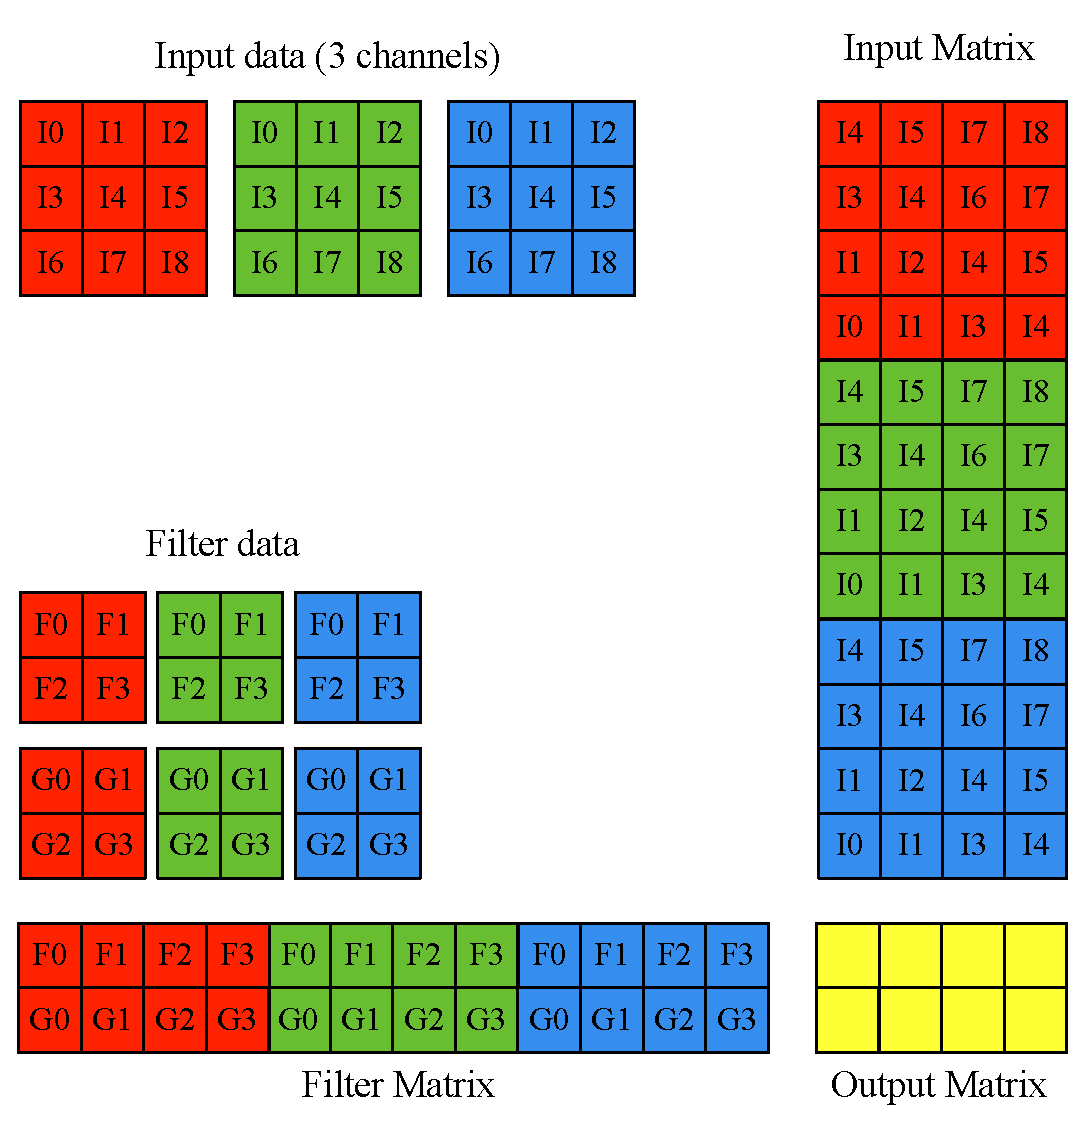
\includegraphics[width=0.75\columnwidth,height=6cm]{./figure/convlowering.eps}
  \caption{An example (reproduced from \cite{ChetlurWVCTCS14}) of converting a simple convolution into matrix multiplications. Here, two filters are used to convolve with a 3-channel input.}
  \label{fig:convlowering}
\end{figure}

{\color{red} Several algorithms, including FFT-based and Winograd-based convolutions, have been proposed to optimize the convolution
operation. All these approaches require to transform 4D tensors into the desired matrix, thus incurring high memory overhead. Figure
\ref{fig:convlowering} illustrates how to translate a simple convolution into matrix multiplications. A filter is typically organised as
4-element tuple, $(batch\_size, chanel\_size, height, width)$. For example, the data dimension of the filter in Figure
\ref{fig:convlowering} is $(2, 3, 2, 2)$. We can see that the transformed filter matrix has the same number of elements as the filter data.
The input data dimension is (1, 3, 3, 3) and 27 elements in total, whereas the input matrix has 48 elements and 44\% of which are redundant
elements. This can incur numberous memory transactions. The experiments (Table \ref{tab:3dtrans}) show that our approach reduce the number
of memory transactions by a factor of 4.4 compared with GEMM-based 3D convolution.}


%\subsection{Overview of Our Approach}
\begin{figure}[t!]
\centering
  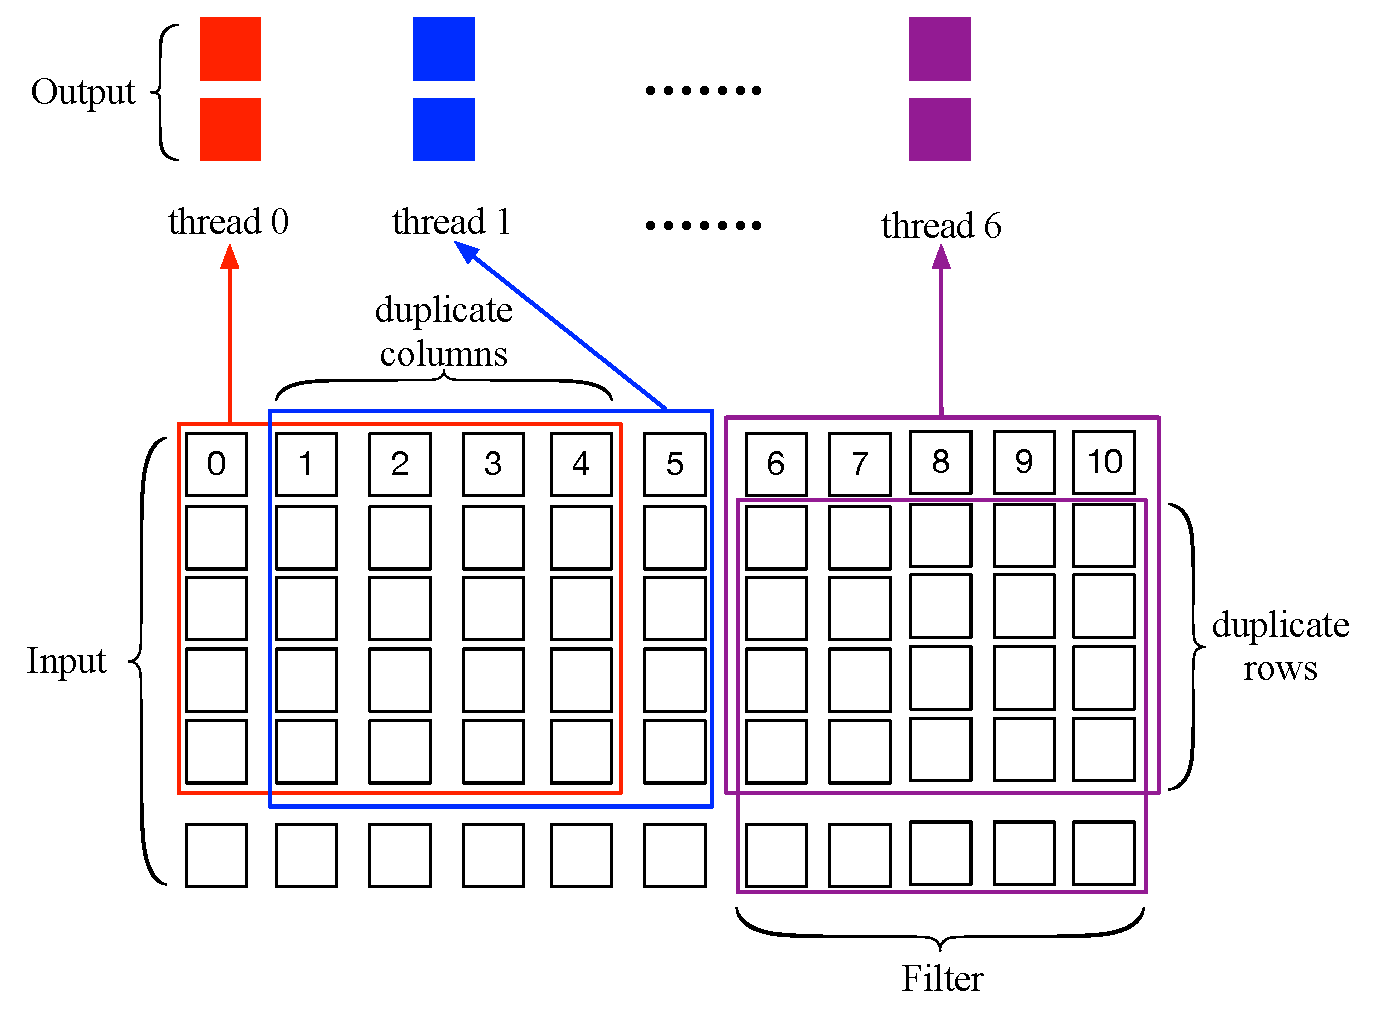
\includegraphics[width=\columnwidth,height=6cm]{./figure/twostrategies.eps}
  \caption{Example of performing 2D convolution using a GPU. Here, the filter size is $5 \times 5$, the input image size is $6 \times 11$
  and the output size is $2 \times 7$. Each thread calculates one column of the output. Assume threads 0 and 1 load the required regions from input
  image with four duplicate columns, and thread 6 loads two overlapped regions from input image and generates four duplicate rows. Numbers in
  the square denote the index of input elements.}
  \label{fig:twostrategies}
\end{figure}

\section{Memory Transaction Optimization}
\label{sec:strategies} 
{\color{red}We take the 2D convolution shown in Figure \ref{fig:twostrategies} as an example to demonstrate how to optimize convolution operations.}
%As a motivation example, consider Figure \ref{fig:twostrategies} that shows a simple 2D convolution executing on a GPU. 
Here, we slide a $5 \times 5$ filter over a $6 \times 11$ image to produce a $2 \times 7$ output. In this example, each thread calculates one column of the output. For example, threads 0 and 1 could execute code to slide the filter along the width dimension. Both threads load two overlapped regions from the input image, thereby generating four duplicate columns. Assume thread 6 demonstrates the process of sliding the filter along the height dimension. It loads two overlapped regions and generates four duplicate rows.

%Our approach can eliminate redundant elements on the column and the width dimensions to reduce the number of memory accesses.  In the proposed column reuse algorithm, we let each thread load the required first and last columns and retrieve the remaining from other threads through shuffle instructions. The difference in the usage of shuffle instructions between our algorithms and the previous study \cite{vasilache2014fast} is discussed in Section \ref{sec:strategies}. In the proposed row reuse algorithm, we let each thread load overlapped rows only once and multiply each row with multiple rows of a filter to calculate multiple output elements. A major performance issue encountered in our implementation is that the thread local arrays with dynamic indexing are placed in the local memory, which possesses the same access latency as the global memory. To solve this problem, we use pack and unpack operations to transform dynamic indexing into static indexing.

Our approach optimizes convolution operations on GPUs by reusing column and row elements. Before getting to details, we first give the notations used in the remaining chapters in Table \ref{tab:notations}.

\begin{table}[H]
\caption{Notations for the convolution operation.}
	\begin{tabular}{c|c}
	\hline
		$I$, $F$, $O$ & Input, Filter, Output \\
		\hline
		$N$, $C$, $H$, $W$ & batch size, channel, height, width\\
		\hline
	\end{tabular}
	\label{tab:notations}
\end{table}

%In this paper, we use $I$, $F$ and $O$ to denote an input, a filter and an output tensor respectively. Each tensor is indexed according to its batch size ($N$), channel ($C$), height ($H$) and width ($W$). For example, $I_N$, $I_C$, $I_H$ and $I_W$ represent the batch size, number of channels, width and height of an input, $I$.

\subsection{Column Reuse}
\label{sec:creuse}
\begin{figure*}[t!]
	\begin{subfigure}{0.33\textwidth}
		\centering
		\captionsetup{width=0.9\textwidth}
		 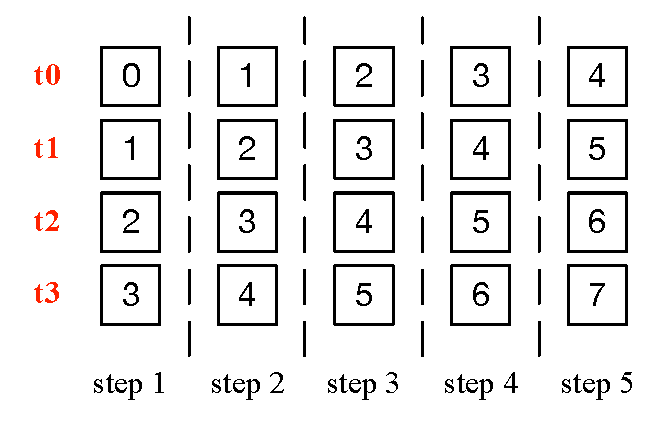
\includegraphics[width=0.98\textwidth,height=4.5cm]{./figure/directconv.eps}
		 \caption{Direct convolution: Each thread loads 5 input elements from global memory.}
		 \label{fig:directalgo}
	\end{subfigure}
	\begin{subfigure}{0.3\textwidth}
		\centering
		\captionsetup{width=0.9\textwidth}
		 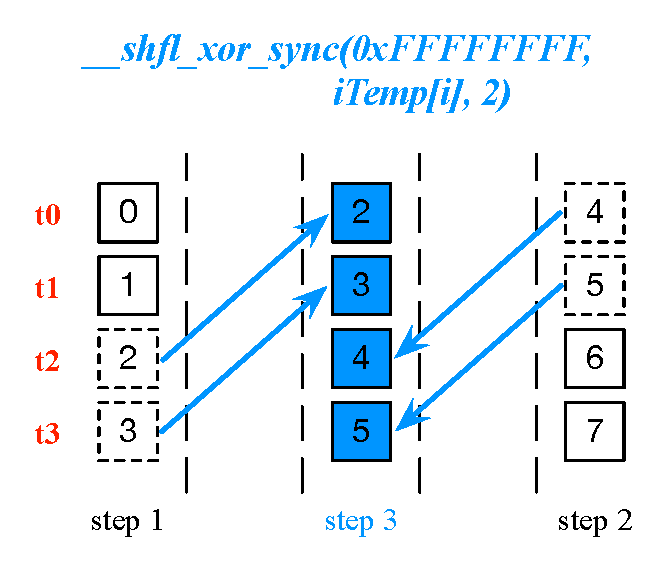
\includegraphics[width=\textwidth,height=4.5cm]{./figure/optalgo1.eps}
		 \caption{Optimized convolution: each thread retrieve its third element from the corresponding thread.}
		 \label{fig:optalgo1}
	\end{subfigure}
	\begin{subfigure}{0.3\textwidth}
		\centering
		\captionsetup{width=0.9\textwidth}

		 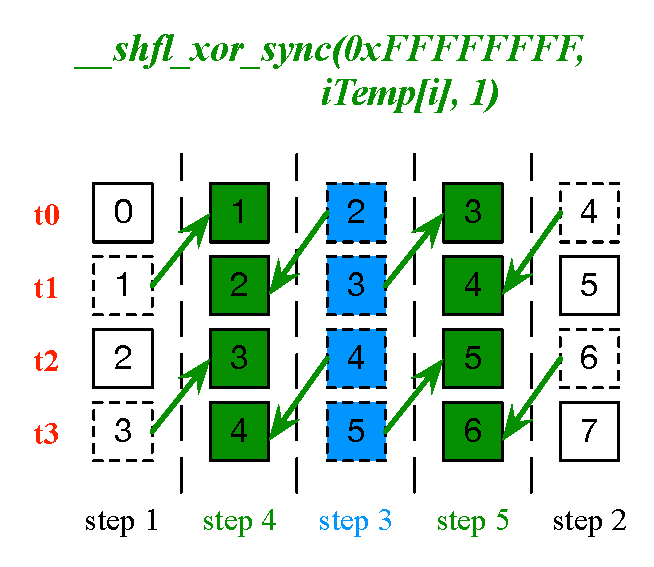
\includegraphics[width=0.96\textwidth,height=4.5cm]{./figure/optalgo2.eps}
		 \caption{Optimized convolution: each thread retrieve its second and fourth elements from corresponding threads.}
		 \label{fig:optalgo2}
	\end{subfigure}
  \caption{Illustration of direct and optimized convolution. We use a $5 \times 5$ filter  and each thread calculate convolution for one output element. Here we demonstrate how each thread processes first 5 corresponding input elements.}
   \label{fig:corealgo}
\end{figure*}



Figure \ref{fig:corealgo} depicts our column reuse algorithm, which consists of a number of step.

 In step 1 of Figure \ref{fig:directalgo}, each thread loads the first corresponding input elements from the
global memory. Given that the addresses of these elements are contiguous (0, 1, 2, 3), the memory controller can coalesce the accesses into
one memory transaction. Therefore, five memory transactions are required for steps 1-5 of. Each pair of adjacent threads have four
duplicate input elements, which corresponds to the duplicate columns in Figure \ref{fig:twostrategies}.

The input elements 1, 2 and 3 loaded in step 2 would have already been loaded by threads $t1$, $t2$ and $t3$ in step 1 (Figure
\ref{fig:directalgo}). Therefore, we can retrieve the input elements 1, 2 and 3 from the threads $t1$, $t2$ and $t3$ instead of loading
them from the global memory (or L1 cache). This kind of duplication also occurs in steps 3, 4 and 5.

To eliminate the redundant loads, we use the shuffle instructions to exchange input elements among different threads. In steps 1
and 2 of Figure \ref{fig:optalgo1}, each thread loads the corresponding first and fifth input elements from the global memory. In step 3, each
thread utilizes the shuffle instruction to retrieve the third element from another thread. Threads $t0$ and $t1$ retrieve the third elements
from threads $t2$ and $t3$, respectively, and provide the fifth elements (dashed squares in step 2) for both threads.
Similarly, threads $t2$ and $t3$ retrieve the third elements from threads $t0$ and $t1$, respectively, and provide the first
elements (dashed squares in step 1) for threads $t0$ and $t1$. This exchange process can be implemented using the instruction
$shfl\_xor(iTemp[i],2)$ (taking CUDA shuffle as an example, \cite{CUDAtoolkit} provides the exact form of the shuffle instructions), where $iTemp$ is the thread local
array used to store the five input elements, and $i$ indexes which element to provide. For threads $t0$ and $t1$, both need to provide the fifth
elements, thus $i=4$. For threads $t2$ and $t3$, both need to provide the first elements, thus $i=0$. The procedure presented in Figure  \ref{fig:optalgo2} is the same as that in Figure \ref{fig:optalgo1}, except that each thread in Figure 3c retrieve itsthe former retrieves the second and fourth elements from its neighboring threads.

However, the instruction $shfl\_xor(iTemp[i],2)$ significantly degrades the performance of the convolution because $iTemp$ is an array with
dynamic indexing, which means that the compiler cannot decide which element to provide at the compile time. Therefore, the compiler
places array $iTemp$ in the local memory, which possesses the same access latency as the global memory, instead of the registers. This process significantly increases the memory access time and degrades the performance of the convolution.

\begin{figure}
	\centering
	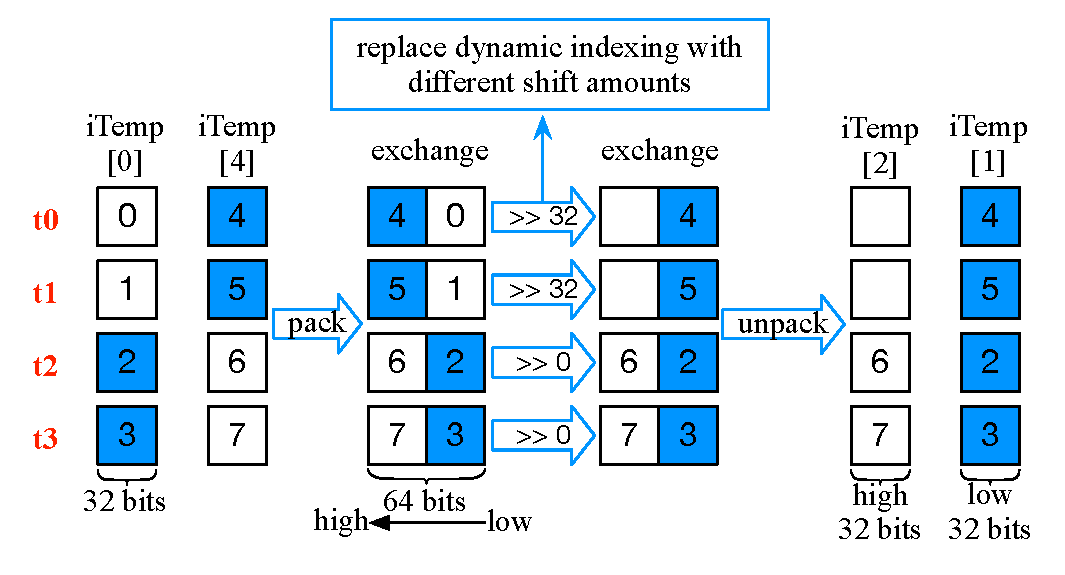
\includegraphics[width=\columnwidth,height=4.5cm]{./figure/exchange.eps}
\caption{Convert the dynamic indexing of array $iTemp$ into static indexing. Therefore, The compiler can put $iTemp$ into registers instead of local memory.}
\label{fig:exchange}
\end{figure}


\begin{algorithm}
	$tid \gets threadIdx.x$\;
	$iTemp[0] \gets iData[iIndex]$\;
	$iTemp[4] \gets iData[iIndex+4]$\;
	$mov\ exchange, \{iTemp[0], iTemp[4]\}$\;
	$shift \gets ((tid+2)\&2)<<4$\;
	$exchange \gets exchange >> shift$\;
	$mov\ \{iTemp[1],iTemp[2]\}, exchange$\;
	$iTemp[2] \gets shfl\_xor(iTemp[1],2)$\;	
	
	\caption{Data exchange algorithm for retrieving the third element}
	\label{algo:basic}
\end{algorithm}

To convert dynamic indexing into static one, we design Algorithm \ref{algo:basic} for step 3 in Figure \ref{fig:optalgo1} and
Algorithm \ref{algo:basic2} for steps 4 and 5 in Figure \ref{fig:optalgo2}. Both algorithms use the same method but deal with different
situations. Moreover, both algorithms can change dynamic indexing into static indexing and reduce the number of memory accesses. We then use Algorithm
\ref{algo:basic} as an example to illustrate the elimination of dynamic indexing.

Figure \ref{fig:exchange} illustrates the process of Lines 4-7 of Algorithm \ref{algo:basic}. First, each thread loads the corresponding first and fifth input elements into $iTemp$ (Lines 2-3). Second, the 32-bit elements are packed into a 64-bit variable $exchange$, where $iTemp[4]$ and $iTemp[0]$ are the high and low 32 bits, respectively (Line 4). The exchange is right-shifted by 32 to place $iTemp[4]$ in the low 32 bits because threads $t0$ and $t1$ must provide the fifth
elements, which are the high 32 bits of $exchange$. Threads $t2$ and $t3$ must provide the first elements, which are already the low 32 bits of $exchange$. Therefore, we right shift $exchange$ in threads $t2$ and $t3$ by 0. The shift amounts of each thread is calculated on the basis of the thread ID (Line 5). Third, unpack $exchange$ into $iTemp[2]$
(high 32 bits) and $iTemp[1]$ (low 32 bits) (Line 7). And $iTemp[1]$ is the element that each thread must provide. Lastly, the
shuffle instruction is used to exchange the elements among the threads (Line 8).

In contrast to the previous usage of shuffle instructions \cite{vasilache2014fast}, Algorithm \ref{algo:basic} successfully replace dynamic
indexing $i$ in $shfl\_xor(iTemp[i],2)$ with static indexing $1$ in $shfl\_xor(iTemp[1],2)$. Algorithm \ref{algo:basic} successfully
eliminates dynamic indexing and therefore all thread local variables can be put in registers, which significantly improve the performance
of convolution.

\begin{algorithm}[t!]
	$tid \gets threadIdx.x$\;
	$mov\ exchange, \{iTemp[0], iTemp[2]\}$\;
	$shift \gets ((tid+1)\&1)<<5$\;
	$exchange \gets exchange >> shift$\;
	$mov\ \{iTemp[0],iTemp[1]\}, exchange$\;
	$iTemp[1] \gets shfl\_xor(iTemp[0],1)$\;	
	\caption{Data exchange algorithm for retrieving the second element}
	\label{algo:basic2}
\end{algorithm}

Steps 4 and 5 in Figure \ref{fig:optalgo2} have similar procedure as step 3 in Figure \ref{fig:optalgo1}. Thus, we slightly modify
Algorithm \ref{algo:basic} to obtain Algorithm \ref{algo:basic2}. The main distinction between the two algorithms is that four threads are involved to exchange the
elements in Figure \ref{fig:optalgo1}, whereas only two adjacent threads are involved in Figure \ref{fig:optalgo2}. Therefore, the shift amounts for each thread (Line 3) should be recalculated, and the arguments of the shuffle instruction (Line 6) should be changed.

In summary, Algorithms \ref{algo:basic} and \ref{algo:basic2} can reduce the number of memory transactions from 5 to 2 and 25 to 10 when 5 and 25 input elements are loaded, respectively. This reduction greatly improves the performance of the convolution.

\subsection{Row Reuse}
\label{sec:rowreuse}
\begin{figure}
	\centering
	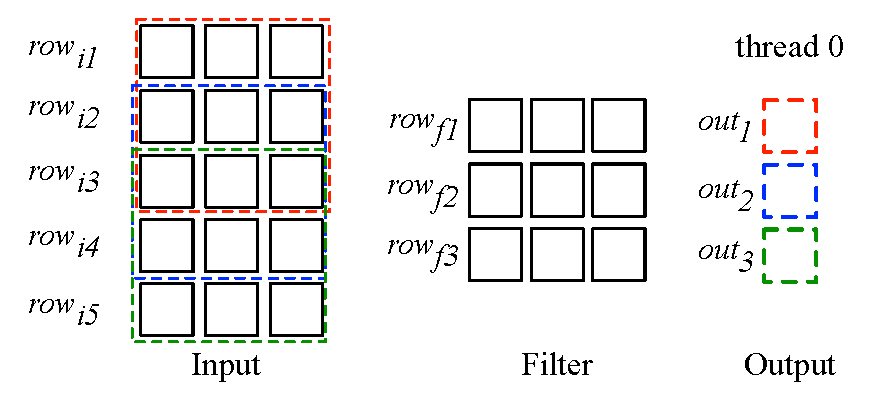
\includegraphics[width=\columnwidth,height=3.7cm]{./figure/rowreuse.eps}
\caption{A $3 \times 3$ filter is used to slide over the input image along height dimension and produce a column of output elements. One thread is used to calculate this column of output elements.}
\label{fig:rowreuse}
\end{figure}

Figure \ref{fig:rowreuse} shows that when sliding the filter over the input image along the height dimension, we can obtain a column of the output elements. Our design then uses one thread to calculate one column of the output elements. Based on Figure \ref{fig:rowreuse},
we can perform convolution as follows:

\begin{gather*}
  out_1=row_{i1} \cdot row_{f1} + row_{i2} \cdot row_{f2} + row_{i3} \cdot row_{f3} \\
out_{2}=row_{i2} \cdot row_{f1} + row_{i3} \cdot row_{f2} + row_{i4} \cdot row_{f3} \\
	out_{3}=row_{i3} \cdot row_{f1} + row_{i4} \cdot row_{f2} + row_{i5} \cdot row_{f3}
\end{gather*}

The above equations suggest that $row_{i2}$ and $row_{i4}$ are loaded twice, and $row_{i3}$ is loaded three times; nice rows should be loaded in total. To eliminate row duplications, we redesign the execution of the convolution. After loading a row from the input, we determine the number of output elements that need the row. For example, $out_1$ needs $row_{i1}$, and $out_1$ and $out_2$ need $row_{i2}$. Then, we use
this row to do inner product with corresponding rows of the filter to calculate the output elements that this row. The resigned formulations are shown as follows:
\begin{equation}\nonumber
\begin{aligned}
load\ row_{i1}:
&\ out_1=row_{i1} \cdot row_{f1} \\
load\ row_{i2}:
&\ out_1 = out_1+row_{i2} \cdot row_{f2}\\
&\ out_2=row_{i2} \cdot row_{f1}\\
load\ row_{i3}:
&\ out_1 = out_1+row_{i3} \cdot row_{f3}\\
&\ out_2 = out_2+row_{i3} \cdot row_{f2}\\
&\ out_{3}=row_{i3} \cdot row_{f1}\\
load\ row_{i4}:
&\ out_2=out_2+row_{i4} \cdot row_{f3} \\
&\ out_3=out_3+row_{i4} \cdot row_{f2}\\
load\ row_{i5}:
&\ out_3=out_3+row_{i5} \cdot row_{f3}
\end{aligned}	
\end{equation}



We can see from above equations that only 5 rows are loaded to calculate output elements. A generalized description of the method is
shown in Algorithm \ref{algo:rowreuse}, where $row$ denotes the row loaded from the input, $index$ denotes the index of $row$, $filter$ denotes
the vector of filter rows and $filter[i]$ means the $i$th row of the filter. Lines 1-5 deal with the first $F_H-1$ rows ($row_{i1}$ and $row_{i2}$ in Figure \ref{algo:rowreuse}), which
are needed by less than $F_H$ output elements. Lines 6-11 deal with the rows that are needed by exact $F_H$ output elements ($row_{i3}$ in
Figure \ref{algo:rowreuse}). Lines 12-17 deal with last $F_H-1$ rows, which are needed by less than $F_H$ output elements ($row_{i4}$
and $row_{i5}$ in Figure \ref{algo:rowreuse}).

\begin{algorithm}
	\KwIn{$row$, $index$, $filter$, $Out$}
	\KwOut{$Out$}
	\If{$index \textless F_H-1$}{
		\For {$i \gets 0$ \KwTo $index+1$}{
			$Out[i] \gets Out[i]+row \cdot filter[index-i]$\;
		}
	}\ElseIf{$index \geq F_H-1$ \textbf{and} $index \textless I_H-F_H+1$}{
		\For {$i \gets 0$ \KwTo $F_H$}{
			$o_{index} \gets index-F_H+1+i$\;
			$Out[o_{index}] \gets Out[o_{index}]+row \cdot filter[F_H-1-i]$\;
		}
	}\Else{
		\For {$i \gets F_H-1$ \KwTo $0$}{
			$o_{index} \gets I_H-F_H+1$\;
			$Out[o_{index}] \gets Out[o_{index}]+row \cdot filter[F_H-i]$\;
		}
	}
	\caption{Row reuse}
	\label{algo:rowreuse}
\end{algorithm}

In summary, Algorithm \ref{algo:rowreuse} eliminates row duplications caused by sliding a filter over the input along height dimension. The
algorithm loads each row of the input exactly once and thus greatly reduces the number of memory transactions.

\subsection{Putting Together}
\label{sec:together}
\begin{figure}
	\centering
	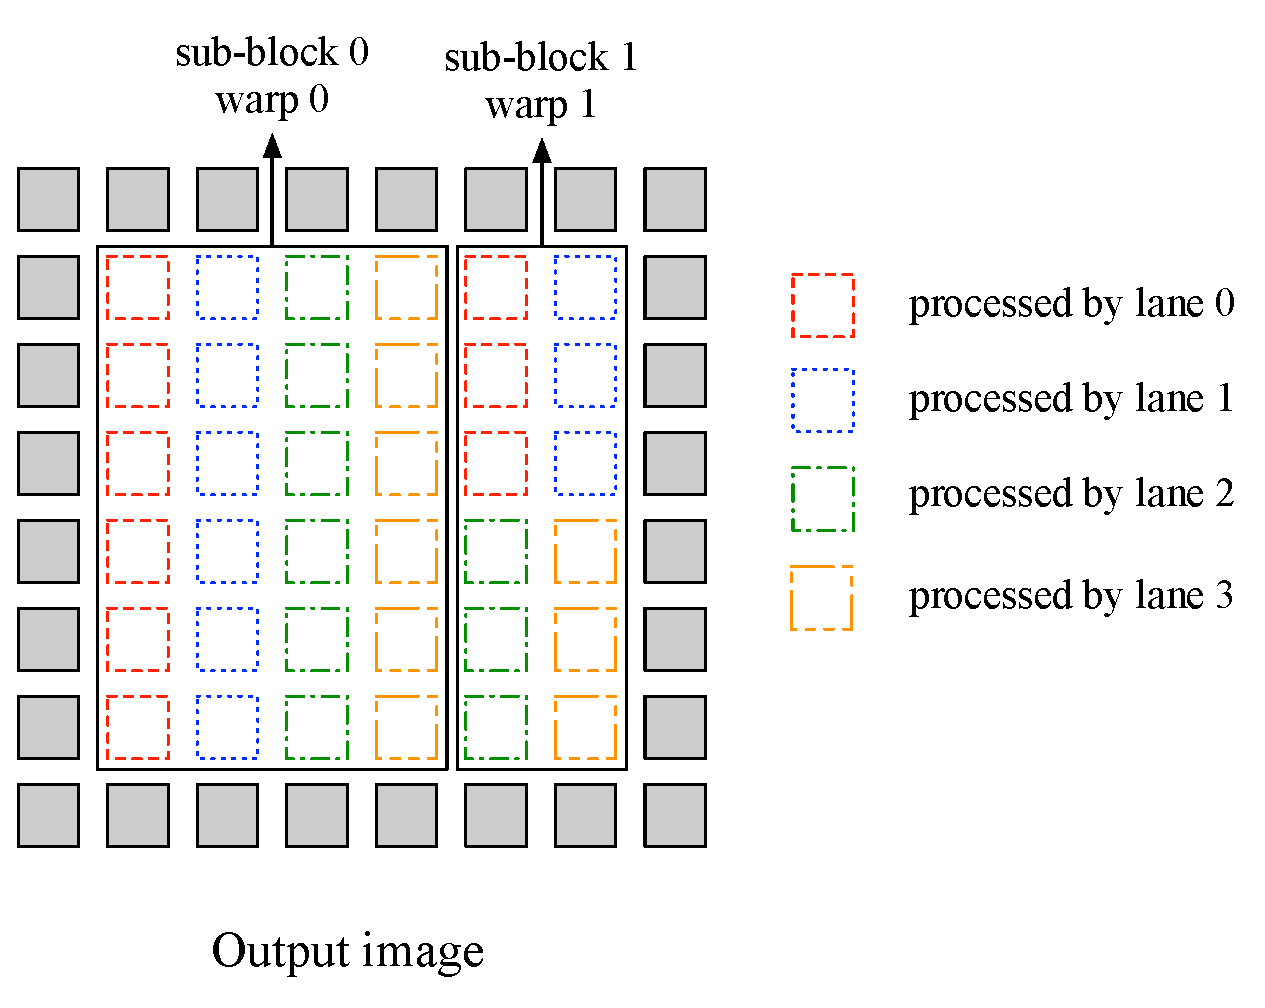
\includegraphics[width=0.8\columnwidth,height=5cm]{./figure/overalldesign.eps} \caption{The output is produced by sliding a $3 \times
3$ filter over an $8 \times 8$ input with one pad. Here, we assume
that the warp size is 4 and thus having $laneid=threadid\%4$.} \label{fig:overalldesign}
\vspace{-2mm}
\end{figure}


We now demonstrate how our column and row reuse optimizations can be used together to optimize GPU memory transactions for convolution
operations. We take the widely used 2D convolution as an example to illustrate how to apply proposed reuse algorithms on convolution
operations.


To apply our approach to 2D convolution, we first divide the output into sub-blocks. Each sub-block contains exactly $n$ columns (in this
work, $n = 32$, which is the default warp size of our GPU platform). The only exception is the last sub-block, which may contain less than
$n$ columns. If a sub-block contains more than $k$ rows ($k=56$ in this work), we then further breakdown the sub-block along the height
dimension. Each GPU thread block will process one or multiple sub-blocks, and each warp will compute one sub-block. As a
result, the threads within the same warp will process the adjacent columns of one sub-block.


\begin{algorithm}[t!]
\small
	\KwIn{$I$, $F$, $subBlockHeight$}
	\KwOut{$O$}
	Load the filter into shared memory\;
	Divide columns of the filter into a combination of 3-column and 5-column sub-filters\;
	$\_\_syncthreads()$\;
	\If{$blockIdx.x \textless gridDim.x-1$}{
		Init thread local register array $sum$ to zero\;
		Calculate the index of the first input element this thread needs, denoted as $inputIndex$\;
		\For{$i \gets 0$ \KwTo $subBlockHeight$}{
			\ForEach{sub-filter}{
				Load corresponding input elements from $inputIndex$ of global memory into $iTemp$\;
				Call $RetrieveThirdElement(iTemp)$ or $RetrieveSecondElement(iTemp)$\;
				Call $RowReuse(iTemp,i,$\textit{sub-filter}$,sum)$\;
			}
			Write completed element of $sum$ into $O$\;
		}		
		
	}
	\Else{
		Divide columns of the last sub-block into multiple partitions and try to evenly assign those partitions to threads of a warp. Each thread uses a direct method to calculate elements of $O$.\;
		The same method is adopted when processing the edge elements of $O$\;
	}
	\caption{2D Convolution Optimization}
	\label{algo:overalldesign}
\end{algorithm}

Figure \ref{fig:overalldesign} shows the mapping process of GPU threads to output elements. In this example, we slide a $3 \times 3$ filter
over an $8 \times 8$ input.  Given that 2D convolutions typically produce an output image with the same size as the input image, the
input image should be padded. To reduce the memory pressure, we do not actually allocate GPU memory space for the padded elements. Instead,
we use different methods to calculate the edge and inner elements of the output. The edge and inner elements are represented by the shaded
and dashed squares in Figure \ref{fig:overalldesign}, respectively.


In this example, we assume each warp contains four threads (Figure \ref{fig:overalldesign}). Therefore, we will divide the inner elements
into multiple sub-blocks and each sub-block contains four columns so that a column can be processed by one of the four GPU threads within a
wrap. In our case, we will have two sub-blocks, where sub-block 0 contains four columns, but sub-block 1 only contains two columns. To
utilize the threads within a warp, we divide elements of the last two columns evenly among the four threads.

\mypara{Generalization.} In Algorithm \ref{algo:overalldesign}, we describe our generalized solution. Here, we process the sub-blocks with
exactly 32 columns (i.e., the default wrap size of our evaluation GPU) and the last sub-block in Lines 4-15 and 16-19, respectively. In
this way, each GPU thread calculates one column of the output elements. This is done through a number of steps. First, each thread block
loads the filter into shared memory and divides the filter into a combination of 3-column and 5-column sub-filters. Next, each thread
calculates the address of the first input element it needs (Lines 6). For each output element and sub-filter, each thread loads
corresponding input elements into $iTemp$ and passes it to Algorithms \ref{algo:basic} and \ref{algo:basic2} to fill the row vector $iTemp$
(Line 10). Then, each thread passes the filled vector $iTemp$ to Algorithm \ref{algo:rowreuse} to calculate multiple output elements and
store results in the register array $sum$ (Line 11). Finally, when the calculation of one output element is completed, we write the
corresponding result in $sum$ into the result array $O$ (Line 13).

\section{Optimizing Pointwise Convolution}
In this section, we first demonstrate how to distribute input channels among threads within a warp. 
Then, we describe how to determine the threads to calculate one input elements.
\subsection{Distribute Input Channels}
Pointwise convolution has a low arithmetic intensity compared with multi-channel 2D convolution. 
Especially when performing training or inference in batch sizes of 64, 32, 16, etc.
However, the pointwise convolution implementation of cuDNN is inefficient in this situation. 
They choose a fixed blocking strategy for convolutions with high and low arithmetic intensity. 
However, blocking strategy which is suitable for high arithmetic intensity will result in GPU underutilization since there is not enough output elements to keep all CUDA cores busy.
To address this problem, we design a dynamic blocking strategy for low arithmetic intensity pointwise convolution that will calculate block size based on output size and hardware limits and yet can hide memory access latency.
The main idea is to let different number of threads to calculate one output elements for different arithmetic intensity.

First, we fix the size of thread block to 4 warps (each warp contains 32 threads). More warps will decrease the block number and may hurt GPU utilization. 
Next, based on the number of SM, we calculate how many output elements each SM needs to process to fully utilize GPU.
The key issue here is to find a value that can increase the arithmetic intensity as well as GPU utilization. 
We give two choices for SM, each SM calculates 2 blocks or 4 blocks, which corresponding to 128 registers per thread or 255 (each thread at most have 255 registers) registers per thread.
We calculate how many output elements each thread block needs to process.
The most difficult part is how to map block tile into warps and threads.
We use two mappings to map thread blocks into output elements.
Now, for each mapping, we can decide how many filters each warp needs to calculate and therefor, how many inputs each warp to calculate.
Now we iterate over all possible channel numbers (1, 2, 4, 8, 16 and 32) to find a filter number that do not exceed half of registers available under this mapping and most close to input number.
Last, we choose the best configurations from all possible ones.
\begin{figure}
	\centering
    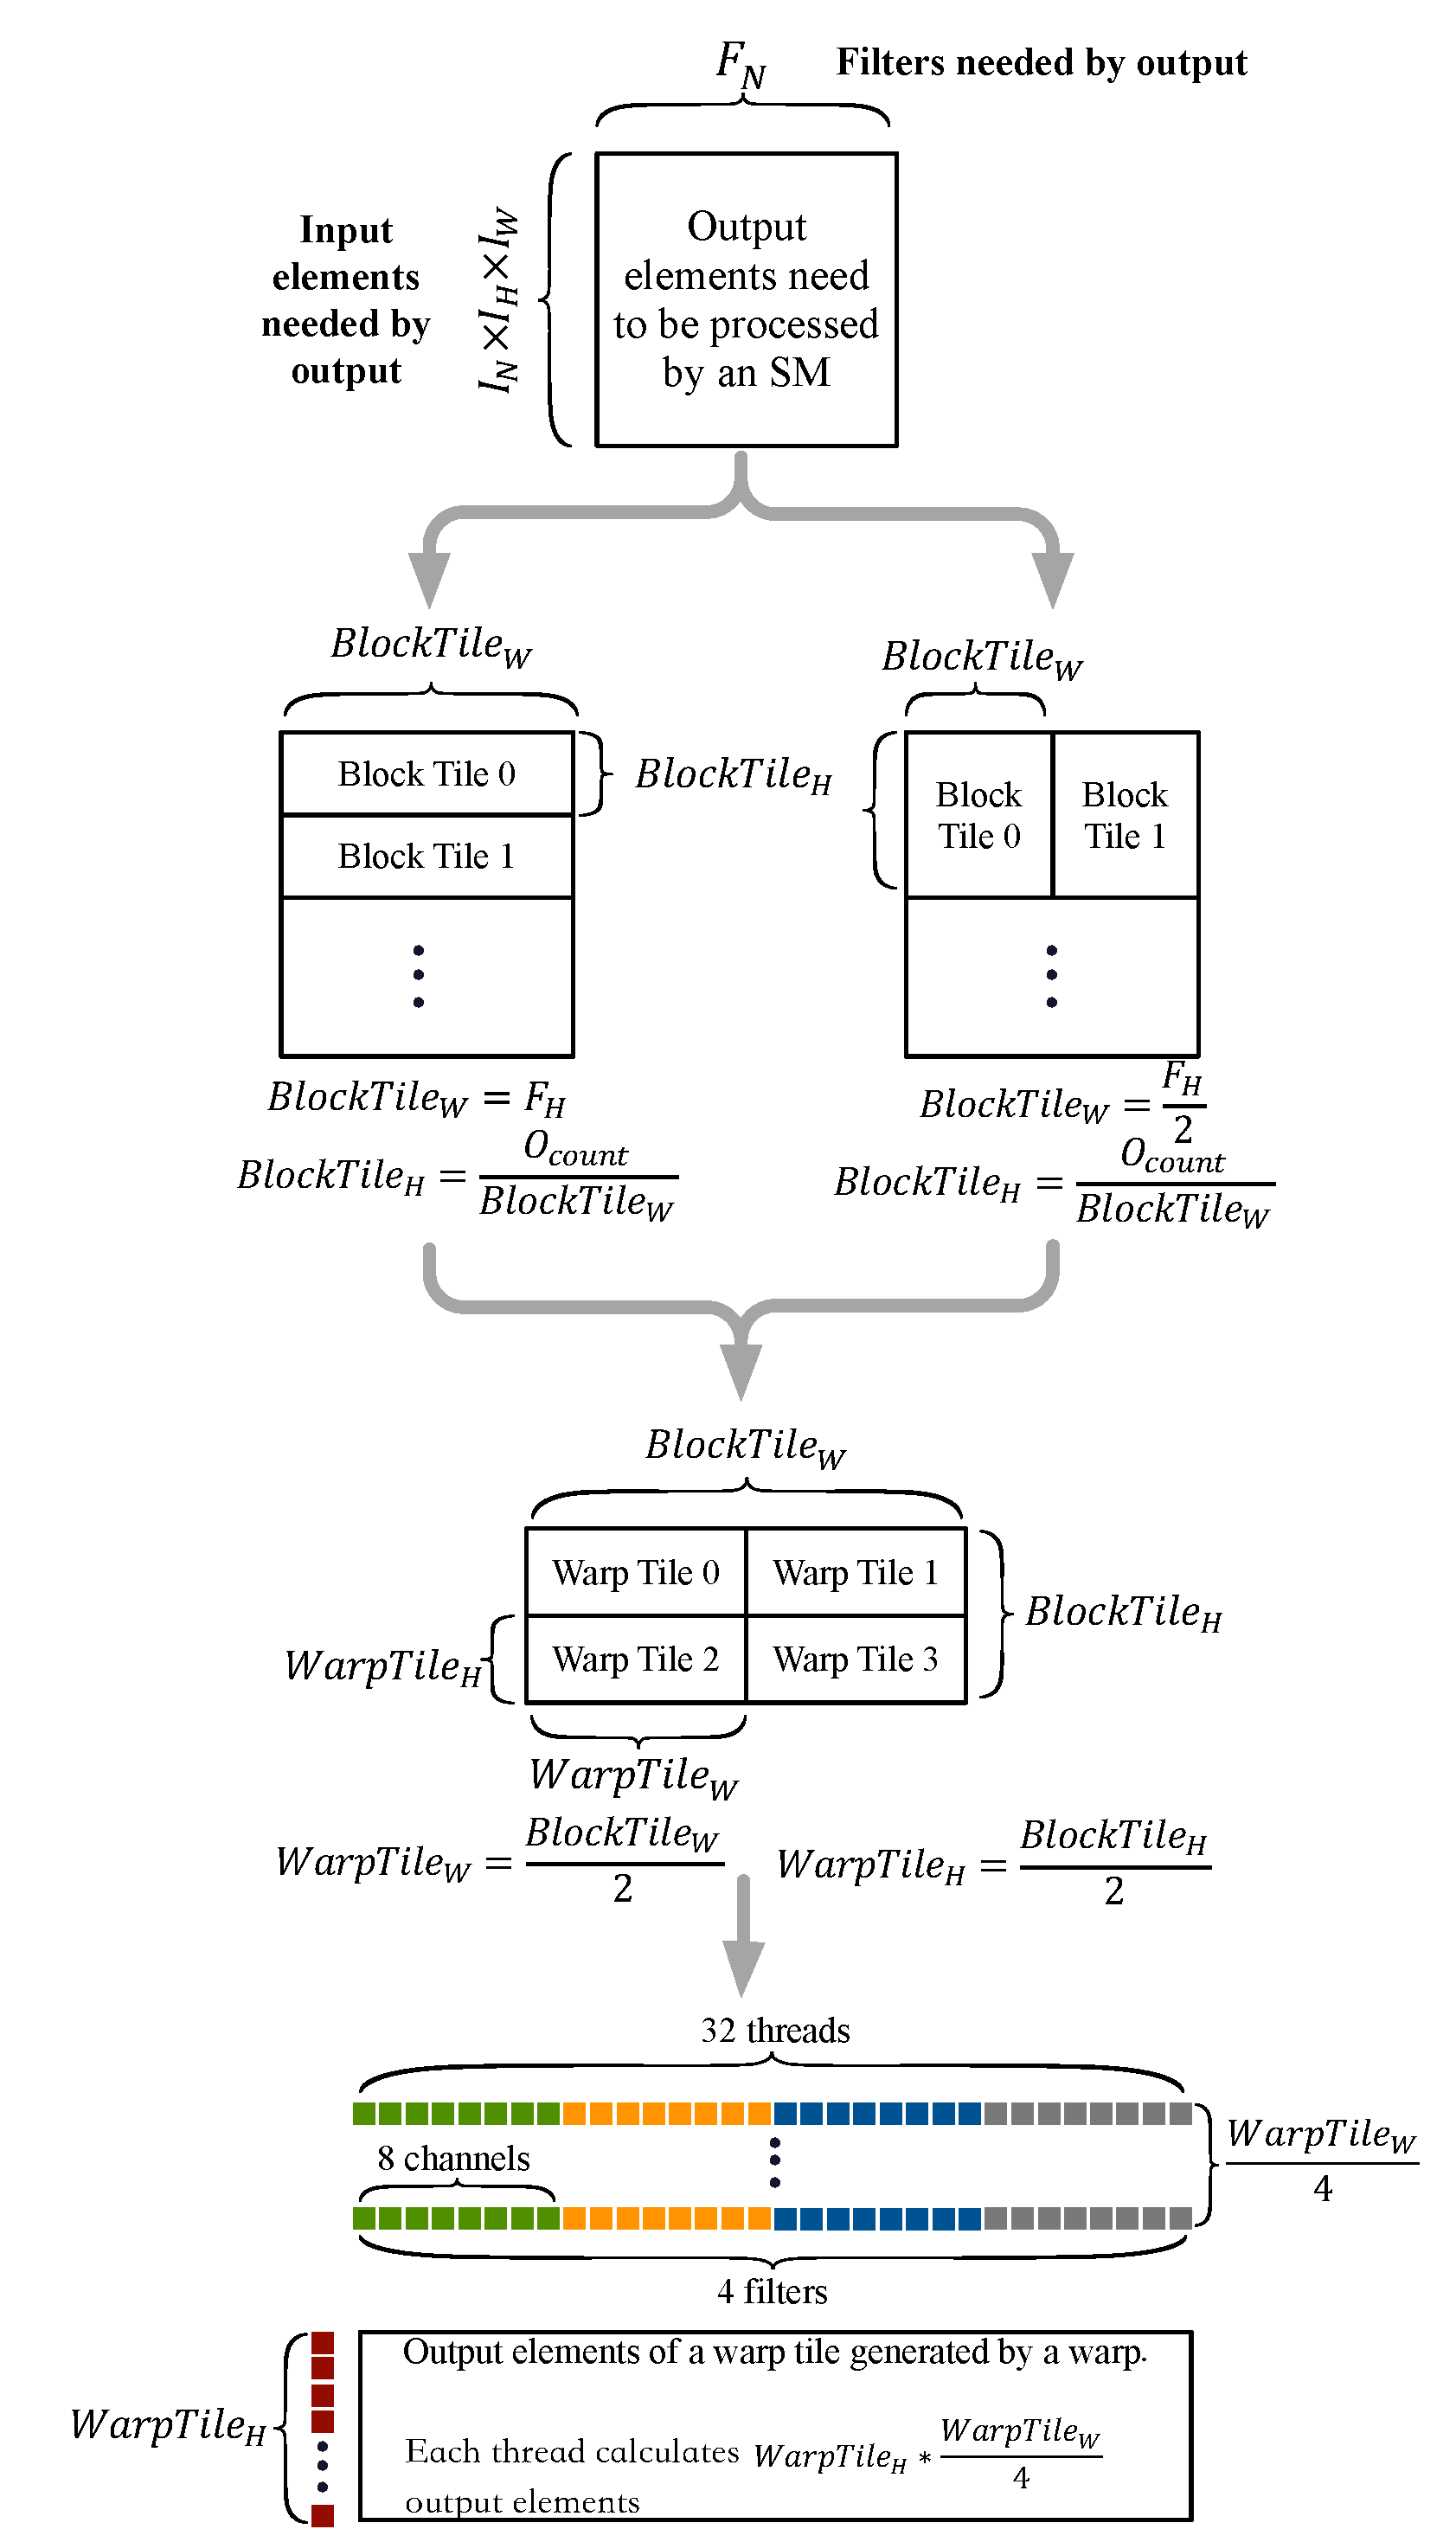
\includegraphics[width=\columnwidth]{./figure/pwflow.eps}
    \caption{} \label{fig:pwflow}
\end{figure}
\begin{algorithm}[t!]
    \small
        \KwIn{$I$, $F$}
        \KwOut{$O$}
        Calculate how many output elements one SM needs to process if we want to fully utilize GPU, denoted as $O_{sm}$\;
        \tcp{below codes are executed on CPU}
        \tcp{we have two options for block tile number, one SM contains 2 or 4 block tiles}
        \ForEach{block tile number of one SM}{
            Use $BlockTile_{count}$ to denote the number of block tiles resided on one SM\;
            \ForEach{block layout}{
                Calculate the width of a block tile, denoted as $BlockTile_W$\;
                $BlockTile_H = \frac{O_{sm}}{BlockTile_W * BlockTile_{count}}$\;
                \If{$BlockTile_H > 32$}{
                    $niter = BlockTile_H/32$\;
                    $BlockTile_H = 32$\;
                }
                $WarpTile_H=\frac{BlockTile_H}{2}$\;
                $WarpTile_W=\frac{BlockTile_W}{2}$\;
                \tcp{there are 6 choices for channel count, 1,2,4,8,16,32}
                \ForEach{channel count}{
                    Use $C_{count}$ to denote how many threads are uesed to calculate channels of the same output element.\;
                    $filter_{num} = \frac{32}{C_{count}}$\;
                    $filter_{num} = \frac{WarpTile_W}{filter_{num}}$\;
                    Calculate registers and shared memory usage under this configuration, and evaluate if the usage not exceeds the limit.\;
                    record the configuration with smallest register usage. 
                }
            }
        }
        \tcp{below codes are executed on GPU}
        All threads in a thread block cooperate to load the needed input and filter into shared memory\;
        $\_\_syncthreads()$\;
        \For{$iter \gets 0$ \KwTo $I_C$ By $C_{count}$}{
            load next $C_{count}$ channels for input and filter into registers\;
            load current channels of input and filter into registers\;
            calculate output elements\;
            write registers of next channels into shared memory\;
        }
        use segmented parallel reduce to get the final output elements and write the result to global memory\;
        \caption{Pointwise Convolution Optimization}
        \label{algo:pwalgo}
\end{algorithm}
\section{Evaluation}
\label{exp}
%We evaluate the implementations on two platforms. The first is the  NVIDIA Tesla K40m, which facilitates 2880 FP32 cores with a 64KB L1 cache and shared memory. The host machine has a 2.40GHz Intel Xeon E5-2620 CPU with 128GB memory and Linux kernel v4.19.85. 
We evaluate the implementations on the NVIDIA RTX 2080 Ti, which facilitates 4350 FP32 cores and 4350 INT32 cores with a 96KB L1 cache and shared memory. The host machine has a 2.30GHz Intel Xeon E5-2697
CPU with 252GB memory and Linux kernel v4.15.0. The platform is shipped with the CUDA Toolkit v10.2. We use the following state-of-the-art image and convolution libraries for comparison:
\begin{itemize}
  \item cuDNN, version 7.6.4. cuDNN is a state-of-the-art convolution implementation that supports 2D and depth-wise convolutions on GPU.
      Moreover, cuDNN can execute GEMM-, FFT- and Winograd-based convolutions.
  \item ArrayFire \cite{Yalamanchili2015}, version 3.6.4. ArrayFire is a popular image and signal processing library. This library implements single-channel 2D convolutions on GPU. ArrayFire uses Just In Time compiling for standard arithmetic operations; thus, the first run of an ArrayFire application takes longer than the second run.
      In the experiment, we run ArrayFire twice in each test and record the second runtime.
  \item NVIDIA Performance Primitives (NPP). NPP is an image and signal processing library. We use NPP for single-channel 2D convolutions only.
  \item GEMM-im2col (im2col). We extract the implementation of the im2col from Caffe \cite{jia2014caffe} and take it as a baseline for the single-channel 2D convolution.
  \item Direct implementation of depth-wise convolution. We implement a direct depth-wise convolution without using the proposed reuse algorithms. We take this implementation as a baseline for depth-wise convolution.

\end{itemize}

%After years of updating, cuDNN has integrated seven widely used convolution algorithms. We use the Therefore, cuDNN provides an option that uses heuristics to find the most suitable algorithm for a convolution. We set the option to $PREFER\_FASTEST$ (the exact option can be found at
%\cite{CUDAtoolkit}); that is, we prefer to use the fastest algorithm regardless of the memory capacity. However, the algorithm selected by the heuristic is not always the fastest. Therefore, we use two types of runtime for cuDNN. One is the real fastest runtime among the seven algorithms and the other is the heuristically fastest runtime. For 2D convolutions, we use the real fastest runtime because two types of runtime are the same.

%Our implementations of convolution use only a small part of shared memory and mainly relay on GPU L1 cache. Therefore we employ $cudaDeviceSetCacheConfig$ function to set GPU cache policy with arguments $cudaFuncCachePreferL1$ for our convolutions.
We run each test case ten times and report the averaged running time. All data are 32-bit float data type and organized as 4D tensors $(N,C,H,$ and $W)$. For
now, we test single-channel 2D and depth-wise convolutions for the filters of size $3 \times 3$ and $5 \times 5$, because small filters are commonly used in applications. The results for the single-channel 2D convolution are presented first in the subsequent section, followed by that for the depth-wise convolution.

\subsection{Single-channel 2D Convolution}
\begin{figure*}
\centering
%\subfloat[Speedups for the filter of size $3 \times 3$ on Tesla K40m.]{\includegraphics[width=\columnwidth,height=6cm]{./figure/2d_norm_f3.eps}
	%\label{fig:2druntimef3c1}}
%\hspace{0em}
%\subfloat[Speedups for the filter of size $5 \times 5$ on Tesla K40m.]{\includegraphics[width=\columnwidth,height=6cm]{./figure/2d_norm_f5.eps}
	%\label{fig:2druntimef5c1}}

\subfloat[Speedups for the filter of size $3 \times 3$.]{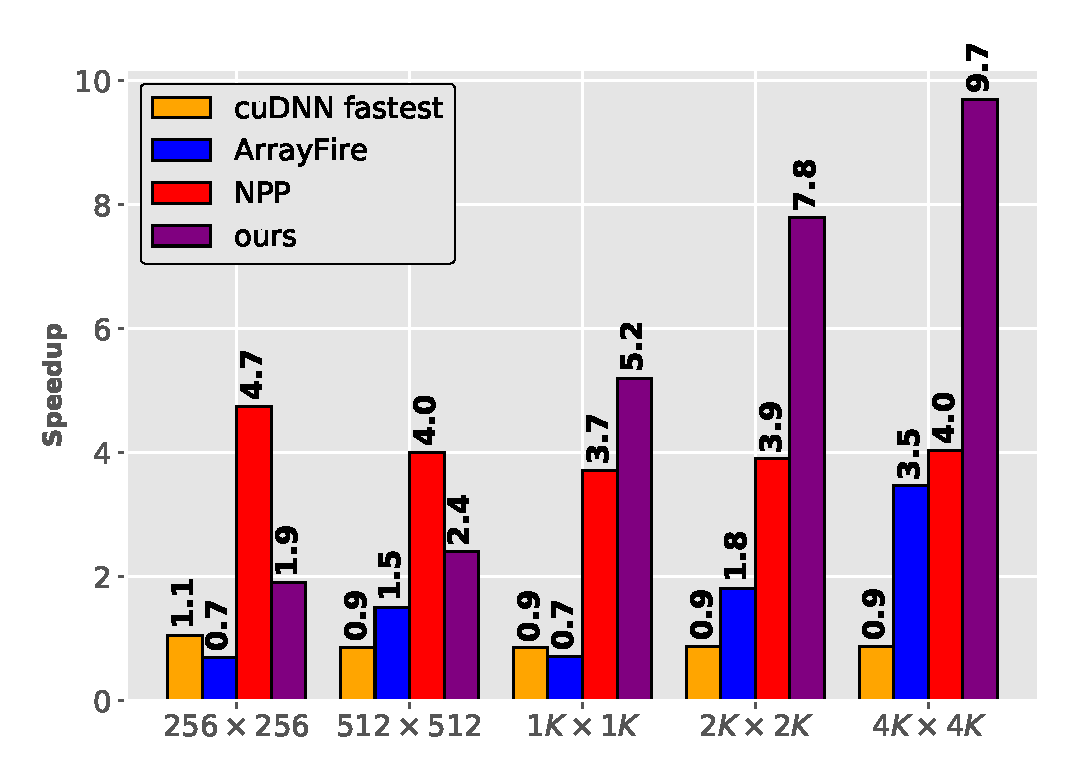
\includegraphics[width=\columnwidth,height=6cm]{./figure/2d_conv_f3.eps}
	\label{fig:2druntimef3c12080}}
\hspace{0em}
\subfloat[Speedups for the filter of size $5 \times 5$.]{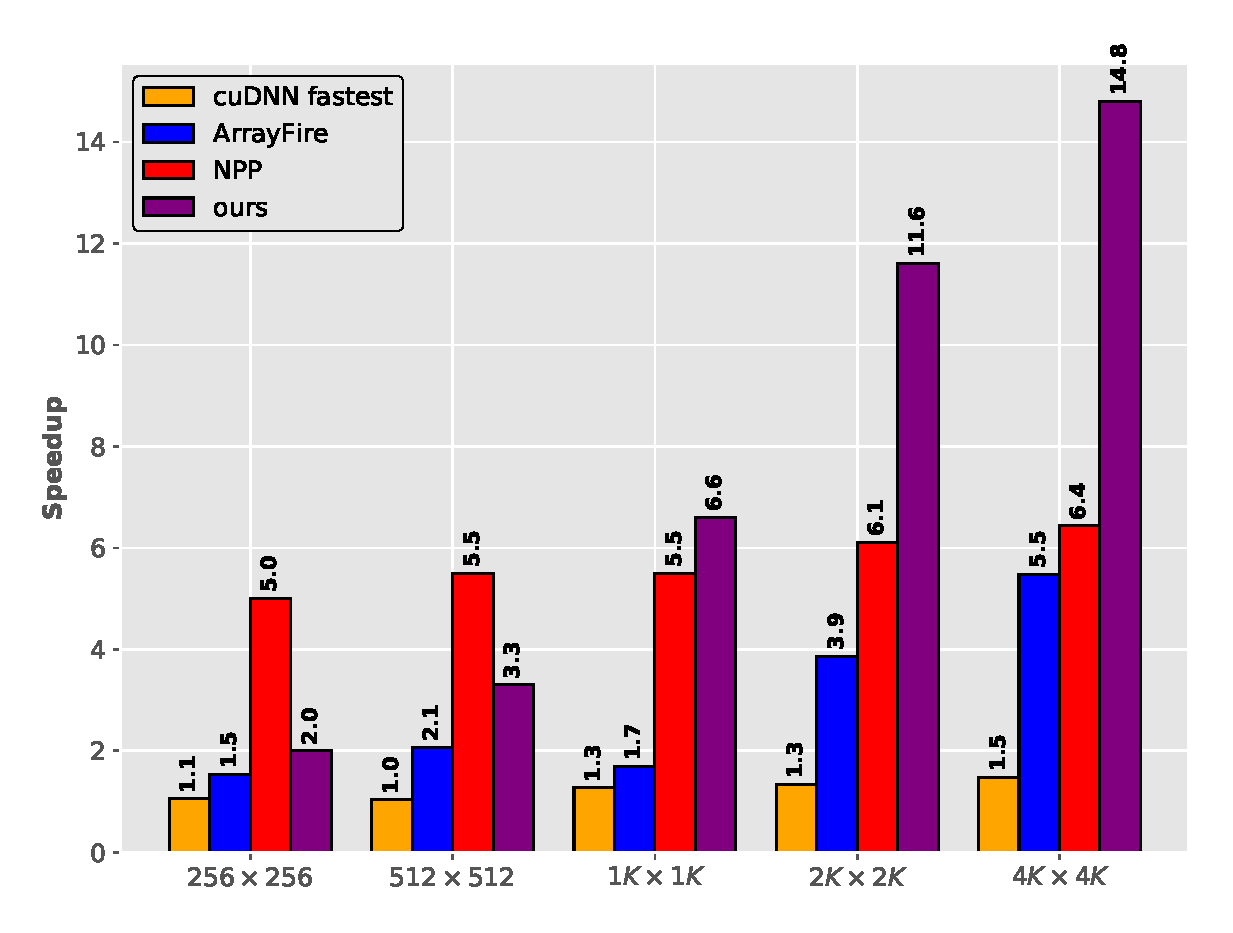
\includegraphics[width=\columnwidth,height=6cm]{./figure/2d_conv_f5.eps}
	\label{fig:2druntimef5c12080}}
	
\caption{Speedups of single-channel 2D convolution of four implementations over im2col on RTX 2080Ti.}
\label{fig:2druntime}
\end{figure*}

%\begin{table*}[]
%\caption{Summation of memory transactions on each type of memory, including global memory, texture memory and shared memory.}
%\label{tab:2dmemtrans}
%\begin{tabular}{c|ccccc|ccccc}
%\hline
%\multicolumn{1}{l|}{}                & \multicolumn{5}{c|}{Filter size $3 \times 3$}                                                & \multicolumn{5}{c}{Filter size $5 \times 5$}                                                \\ \hline
% & $256 * 256$      & $512 * 512$      & $1K * 1K$        & $2K * 2K$        & $4K * 4K$        & $256 * 256$      & $512 * 512$      & $1K * 1K$        & $2K * 2K$        & $4K * 4K$        \\ \hline
%cuDNN                                                  & 6.0E+05          & 2.4E+06          & 9.7E+06          & 3.9E+07          & 1.5E+08          & 1.4E+06          & 5.6E+06          & 2.2E+07          & 8.9E+07          & 3.6E+08          \\
% im2col & 1.1E+05          & 4.4E+05          & 4.4E+05          & 7.0E+06          & 2.8E+07          & 2.3E+05          & 9.3E+05          & 3.7E+06          & 1.5E+07          & 6.0E+07          \\
%im2row & 1.1E+05          & 4.4E+05          & 4.4E+05          & 7.0E+06          & 2.8E+07          & 2.3E+05          & 9.3E+05          & 3.7E+06          & 1.5E+07          & 6.0E+07          \\
%ArrayFire                                              & 4.9E+04          & 2.0E+05          & 7.9E+05          & 3.2E+06          & 1.3E+07          & 1.1E+05          & 4.2E+05          & 1.7E+06          & 6.8E+06          & 2.7E+07          \\
%NPP                                                    & 6.0E+04          & 2.4E+05          & 9.6E+05          & 3.8E+06          & 1.5E+07          & 1.3E+05          & 5.2E+05          & 2.1E+06          & 8.3E+06          & 3.3E+07          \\
%Ours                                                   & \textbf{7.5E+03} & \textbf{2.7E+04} & \textbf{1.1E+05} & \textbf{4.2E+05} & \textbf{1.6E+06} & \textbf{1.0E+04} & \textbf{3.3E+04} & \textbf{1.3E+05} & \textbf{4.9E+05} & \textbf{1.9E+06} \\ \hline
%\end{tabular}
%\end{table*}

This section presents the performance of the single-channel 2D convolution obtained from five implementations, including cuDNN, im2col,  ArrayFire,
NPP and the proposed method. We evaluate the five implementations with the image size ($I_H \times I_W$) ranging from $256 \times 256$ to $4K \times 4K$, $I_N=F_N=1$ and $I_C=F_C=1$. 
%We first present the speedups of four implementation over im2col in Figure \ref{fig:2druntime}. Then we show the effectiveness of our implementation on reducing the number of memory transactions in Table \ref{tab:2dmemtrans}.

Figure \ref{fig:2druntime} presents the speedups of cuDNN, ArrayFire, NPP and our implementation over im2col. The results show that cuDNN is not suitable for single-channel 2D convolutions in contrast to ArrayFire, NPP and the proposed method. The average speedups of cuDNN, ArrayFire, NPP and ours over im2col are 1.09$\times$, 2.2$\times$, 4.9$\times$ and 6.5$\times$, respectively. Our implementation exhibits superior performance over other implementations. Our implementation of the single-channel 2D convolution is derived from direct convolution. We use column (Algorithm \ref{algo:basic}, Algorithm \ref{algo:basic2}) and row reuse (Algorithm \ref{algo:rowreuse}) on direct convolution. Hence, the performance gains are mainly attributed to the reduction on the number of memory transactions.

%Figure \ref{fig:2druntimef3c1} and \ref{fig:2druntimef5c1} present the speedups on Tesla K40m in which the proposed method achieves the best results in nine cases out of ten. Our implementation is  slower than NPP when performing a $3 \times 3$ convolution on a $256 \times 256$ image. The average speedups of our implementation over ArrayFire and NPP on Tesla K40m are 2.1$\times$ and 2.9$\times$, respectively.
%Figure \ref{fig:2druntimef3c12080} and \ref{fig:2druntimef5c12080} show the speedups on RTX 2080 Ti, in which 
In all of ten test cases, the proposed implementation achieves the best results in six cases out of ten. NPP achieves the best results on small image sizes, whereas our implementation demonstrates the best results on large image sizes. We use \emph{nvidia compute} to collect memory profiles, including memory throughput and max bandwidth, of our implementation and NPP when convolving with a $3 \times 3$ filter. The results are shown in Figure \ref{fig:2dmemanaly}.

The average speedup of our implementation for the $5 \times 5$ filter is $7.7\times$, which is better than the speedup for the $3 \times 3$ filter, $5.4\times$. The key reason for this improvement is that, for the $3 \times 3$ filter, there is only one overlapped column and row on width and height dimensions. While for the $5 \times 5$ filter, there are four overlapped columns and rows, therefore column and row reuse algorithms can be used more efficiently compared with  that for the $3 \times 3$ filter.

We can see that as the input size increases, memory throughput and max bandwidth of our implementation exceeds that of NPP, the turning point ($1K \times 1K$ in Figure \ref{fig:2dmemanaly}) is the same as that of speedups in Figure \ref{fig:2druntimef3c12080}, which means that memory performance has a strong relation to the performance of single-channel 2D convolution. Next, we give a detailed analysis of why the memory throughput and max bandwidth of our implementation is low for small input sizes.

When performing single-channel 2D convolutions, only one filter are used to convolve with one single-channel input feature map, which requires much less computation than depth-wise convolutions. Therefore, the memory performance is a deciding factor to the runtime of the single-channel 2D convolution. The proposed row reuse algorithm performs better when a thread calculates more rows of output. However, the more rows each thread calculates, the less warps and thread blocks we can generate. Without enough warps issuing memory requests, the memory throughput and max bandwidth can reduce significantly, which can slow down our implementation. As the input size increases, we can allocate more thread blocks and more warps per thread block. With enough memory requests and reduction on redundant memory transactions, we can increase the memory throughput and max bandwidth, and thus improve the performance of our implementation.

%We use \emph{nvprof} to collect the number of memory transactions for the different types of memories. The GPU global memory is used to store the input data in im2col, im2row, ArrayFire and our implementation. NPP and cuDNN utilize texture memory to store input data, whereas shared memory is normally used to store filter data. Therefore, we sum up the number of read transactions of the three memory types and report the results in Table
%\ref{tab:2dmemtrans}. To save space, we only show the result of the memory transactions collected on Tesla K40m because the result on RTX 2080 Ti exhibits a similar trend.

\begin{figure}
\centering

\subfloat[Memory throughput for the filter of size $3 \times 3$.]{\includegraphics[width=\columnwidth,height=6cm]{./figure/2dmemthroughput.eps}
	\label{fig:2dmemthr}}
\hspace{0em}
\subfloat[Max bandwidth for the filter of size $3 \times 3$.]{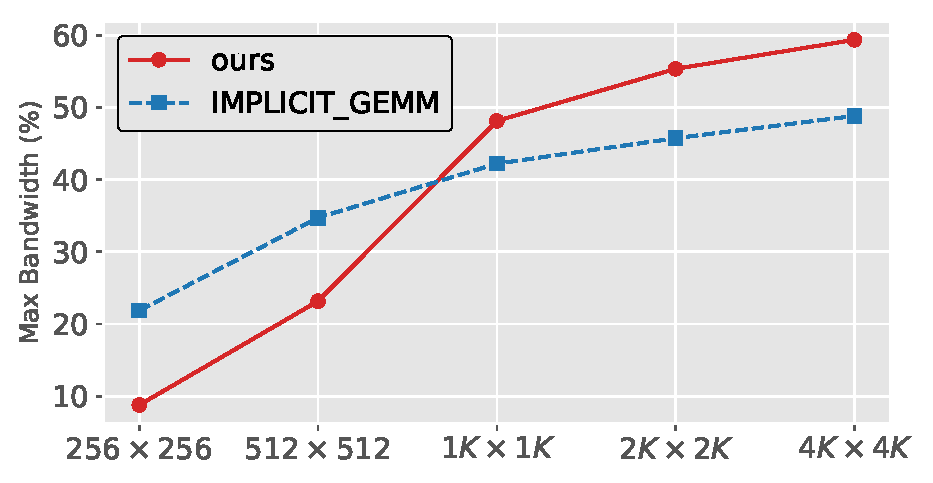
\includegraphics[width=\columnwidth,height=6cm]{./figure/2dmembandwidth.eps}
	\label{fig:2dmaxband}}
	
\caption{Memory analysis of NPP and our implementation for the filter of size $3 \times 3$.}
\label{fig:2dmemanaly}
\end{figure}

%The results in Table \ref{tab:2dmemtrans} verify that our optimization algorithms significantly reduce the number of memory transactions.
%Compared with ArrayFire and NPP, which are well optimized for 2D convolutions, our implementation can respectively reduce the memory transactions by a factor of 10.2 and 12.3 on average.


% Please add the following required packages to your document preamble:
% \usepackage{multirow}


%\begin{table*}[]
%\caption{2d speedup}
%\label{tab:2dspeedup}
%\begin{tabular}{c|ccccc|ccccc}
%\hline
%\multicolumn{1}{c}{}&\multicolumn{5}{c}{$F_H*F_W= 3*3$} &\multicolumn{5}{c}{$F_H*F_W= 5*5$}\\
%\hline
%           & 256*256&512*512&1K*1K&2K*2K&4K*4K&256*256&512*512&1K*1K&2K*2K&4K*4K\\
%\hline
%cuDNN      & 1.91 & 3.74 & 5.69 & 8.07 & 7.72     & 2.86 & 4.86 & 6.08 & 7.40 & 9.20  \\
%im2col     & 1.52 & 3.25 & 5.25 & 7.56 & 7.24     & 2.34 & 4.20 & 5.37 & 6.88 & 8.38  \\
%im2row     & 1.55 & 3.25 & 5.20 & 7.50 & 7.19     & 2.34 & 4.15 & 5.32 & 6.83 & 8.32  \\
%ArrayFire  & 1.23 & 3.67 & 2.59 & 2.37 & 1.95     & 1.40 & 3.12 & 1.73 & 1.43 & 1.57  \\
%NPP        & 0.68 & 1.40 & 2.21 & 3.15 & 3.03     & 1.52 & 2.91 & 3.79 & 4.66 & 5.82 \\
%\hline
%\end{tabular}
%\end{table*}
In summary, our optimization algorithms can significantly reduce the number of memory transactions and improve the performance of single-channel 2D
convolutions. Compared with state-of-the-art image processing libraries, NPP, our implementation achieves average speedups of 1.3$\times$ and 1.28$\times$ for the $3 \times 3$ and $5 \times 5$ filters, respectively.

\subsection{Depth-wise Convolution}
\label{3dconvexp}

\begin{table}[]
\caption{Configurations of 3D convolution}
\label{tab:3dconvconfigs}
\centering
\begin{tabular}{c|ccccc}
\hline
& $I_N$ & $I_C$ & $I_H \times I_W$ &  $F_H \times F_W$ \\
\hline
CONV1 & 512  & 32    & 112*112 & $3 \times 3$, $5 \times 5$  \\
CONV2 & 512  & 96    & 112*112  &$3 \times 3$, $5 \times 5$   \\
CONV3 & 512  & 144   & 56*56  &$3 \times 3$, $5 \times 5$    \\
CONV4 & 512  & 160    & 56*56  &$3 \times 3$, $5 \times 5$    \\
CONV5 & 512  & 192   & 28*28  &$3 \times 3$, $5 \times 5$    \\
CONV6 & 512  & 240   & 28*28  &$3 \times 3$, $5 \times 5$    \\
CONV7 & 512  & 256   & 28*28  &$3 \times 3$, $5 \times 5$    \\
CONV8 & 512  & 384   & 14*14  &$3 \times 3$, $5 \times 5$    \\
CONV9 & 512  & 480   & 14*14  &$3 \times 3$, $5 \times 5$    \\
CONV10 & 512  & 672  & 14*14 &$3 \times 3$, $5 \times 5$     \\
CONV11 & 512  &672  & 7*7 & $3 \times 3$, $5 \times 5$      \\
CONV12 & 512  &960  & 7*7 & $3 \times 3$, $5 \times 5$      \\
CONV13 & 512  &1152  & 7*7 & $3 \times 3$, $5 \times 5$      \\
\hline
\end{tabular}
\end{table}

\begin{figure*}
\centering
		%\centering
		 %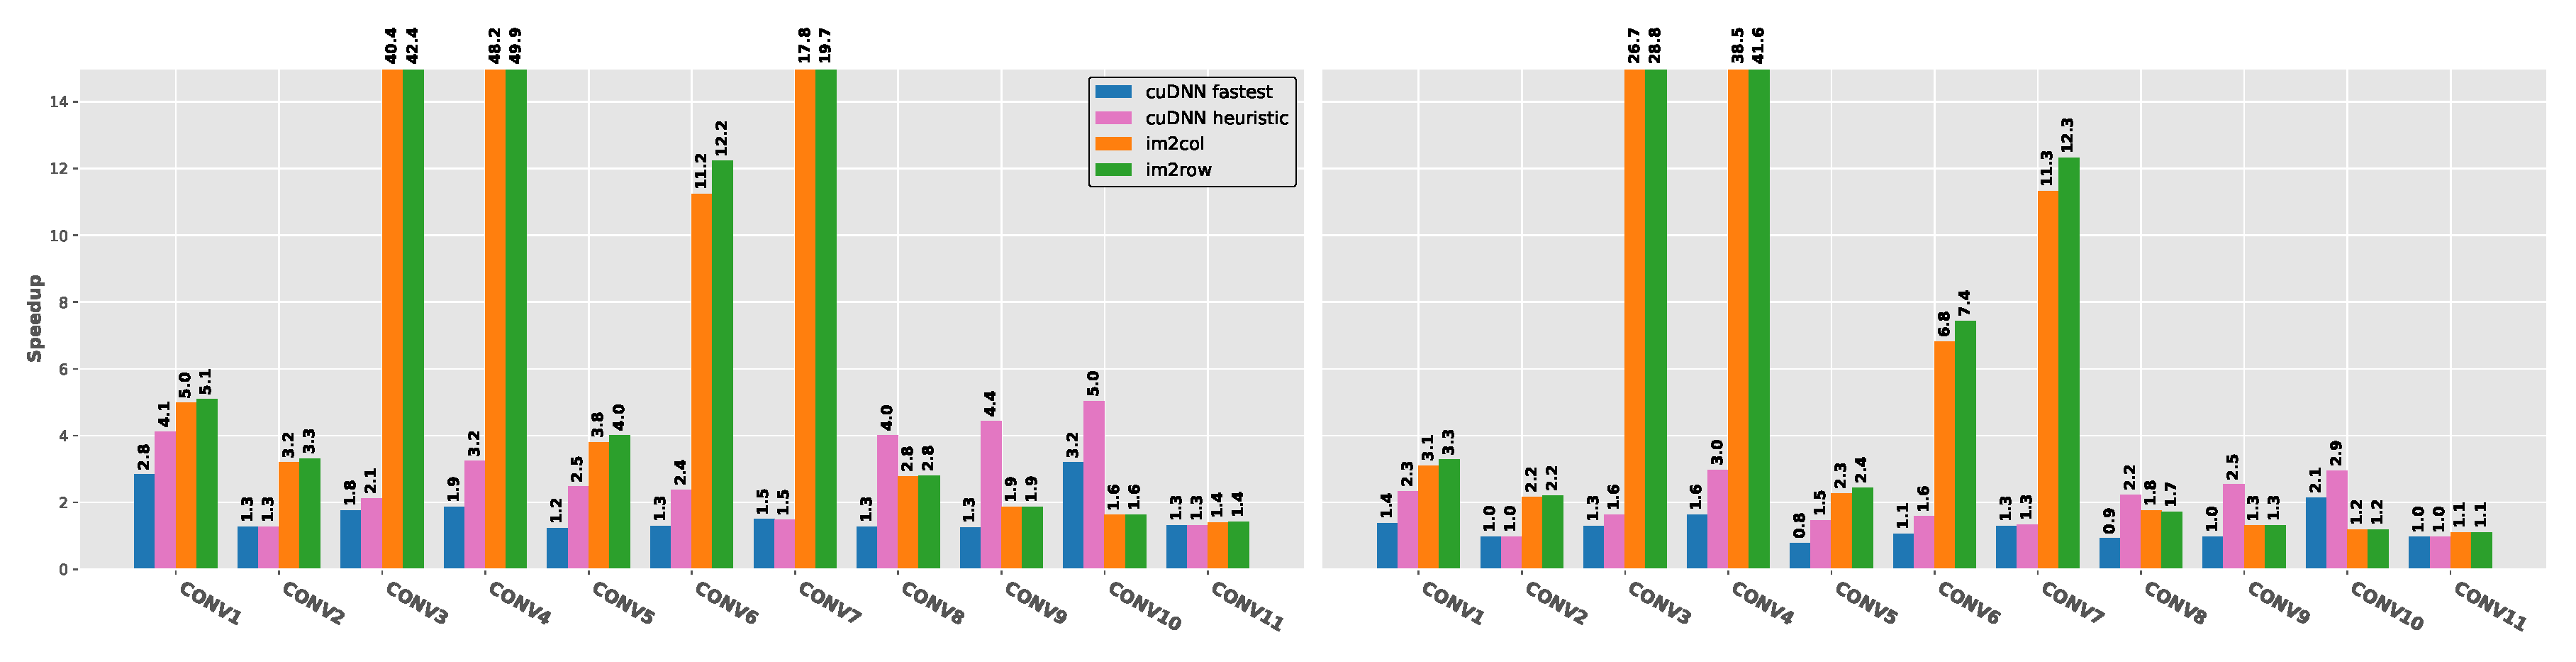
\includegraphics[width=18cm,height=5cm]{./figure/3d_norm_c1.eps}
		 %\caption{Normalized runtime of five implementations for 3D convolution. Left and right parts of the figure is for 3D convolutions with one and three input channels.}
		 %\label{fig:3druntime}
		
%\subfloat[Speedups on Tesla K40m, left is for one channel and right is for three channels.]{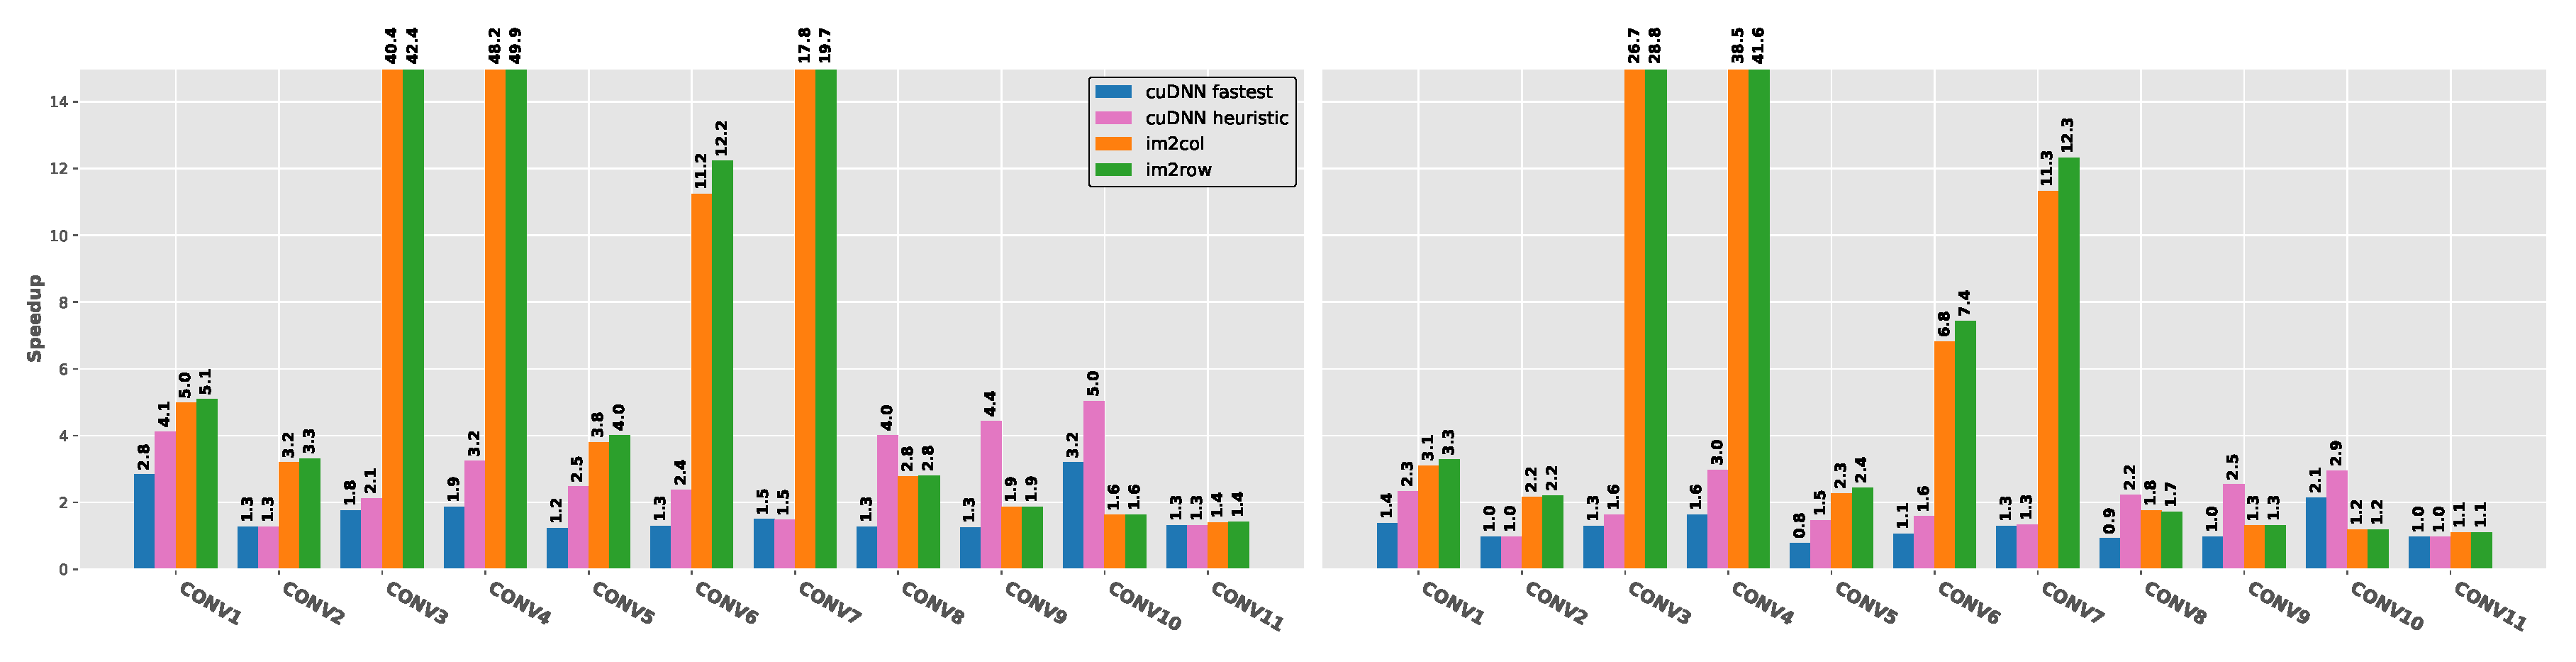
\includegraphics[width=18cm,height=5.7cm]{./figure/3d_norm_c1.eps}
%	\label{fig:3druntimeK40}}
	
\subfloat[Speedups for the filter of size $3 \times 3$.]{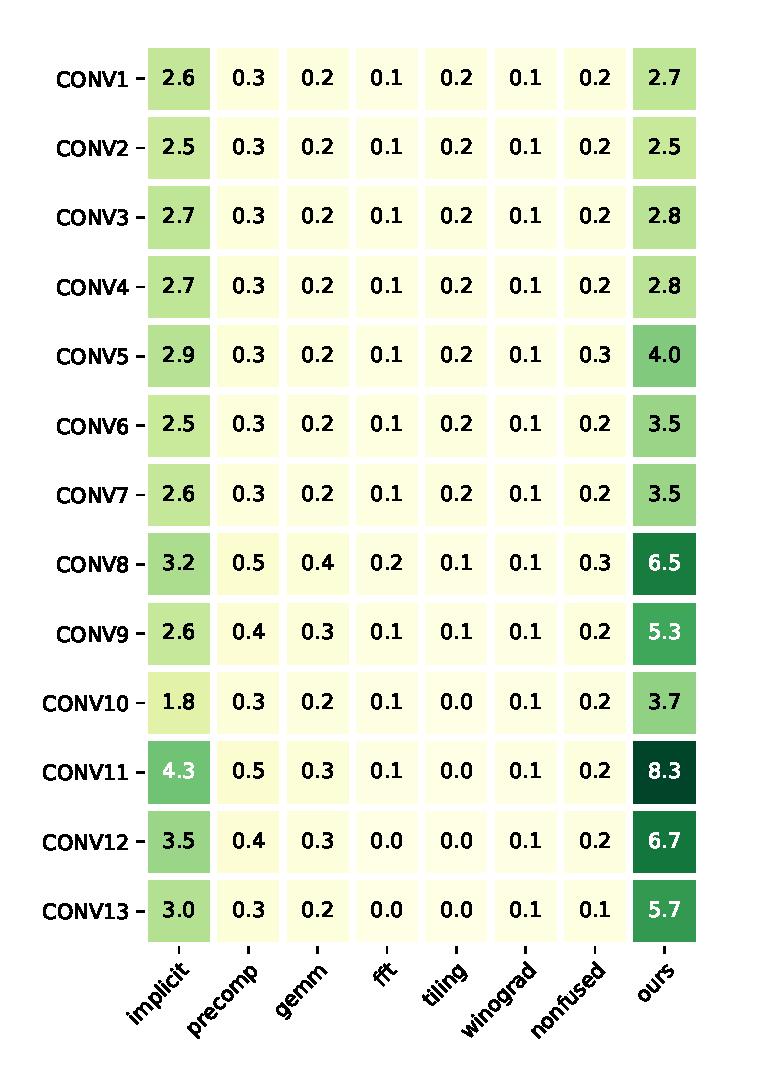
\includegraphics[width=\columnwidth,height=11cm]{./figure/depthwise_f3.eps}
	\label{fig:3druntime2080}}
\subfloat[Speedups for the filter of size $5 \times 5$.]{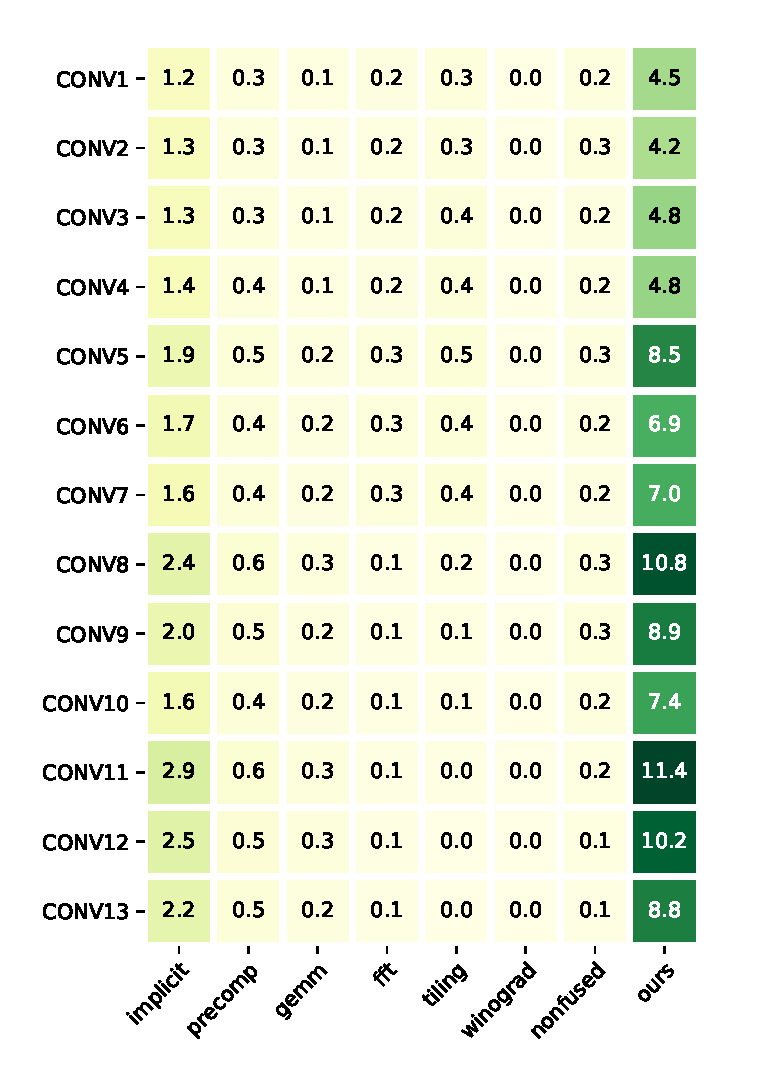
\includegraphics[width=\columnwidth,height=11cm]{./figure/depthwise_f5.eps}
	\label{fig:3druntime2080}}

\caption{Speedups of our implementation and seven cuDNN algorithms over the baseline implementation for the depth-wise convolution.}
\label{fig:3druntime}
\end{figure*}


%\begin{table*}[]
%\centering
%\caption{The number of memory transactions for 3D convolution. Data is collected on Tesla K40m.}
%\label{tab:3dtrans}
%\begin{tabular}{c|ccccc|ccccc}
%\hline
%\multicolumn{1}{l|}{} & \multicolumn{5}{c|}{$I_C=F_C=1$}                                                                                                                                                                                                                                                                  & \multicolumn{5}{c}{$I_C=F_C=3$}                                                                                                                                                                                                                                                                  \\ \hline
%    & \begin{tabular}[c]{@{}c@{}}cuDNN\\ fastest\end{tabular} & \begin{tabular}[c]{@{}c@{}}cuDNN\\ heuristic\end{tabular} & im2col & im2row & \begin{tabular}[c]{@{}c@{}}our 3D\\ conv\end{tabular} & \begin{tabular}[c]{@{}c@{}}cuDNN\\ fastest\end{tabular} & \begin{tabular}[c]{@{}c@{}}cuDNN\\ heuristic\end{tabular} & im2col & im2row & \begin{tabular}[c]{@{}c@{}}our 3D\\ conv\end{tabular} \\ \hline
%CONV1& 1.7E+06& 1.2E+07& 2.3E+06& 2.3E+06& \textbf{8.5E+05}& 3.9E+06& 1.3E+07& 5.5E+06& 5.5E+06& \textbf{2.4E+06}\\
%CONV2& 6.9E+06& 6.9E+06& 4.8E+06& 4.8E+06& \textbf{9.7E+05}& 1.6E+07& 1.6E+07& 1.2E+07& 1.2E+07& \textbf{2.9E+06}\\
%CONV3& 3.5E+05& 1.9E+05& 1.9E+05& 2.5E+05& \textbf{8.4E+04}& 9.5E+05& 5.2E+05& 5.2E+05& 6.8E+05& \textbf{2.5E+05}\\
%CONV4& 2.7E+05& 2.4E+05& 3.0E+05& 3.6E+05& \textbf{2.4E+04}& 7.4E+05& 6.4E+05& 8.0E+05& 9.8E+05& \textbf{7.3E+04}\\
%CONV5& 8.7E+06& 4.5E+06& 5.1E+06& 6.5E+06& \textbf{1.4E+06}& 1.2E+07& 1.2E+07& 1.4E+07& 1.8E+07& \textbf{4.1E+06}\\
%CONV6& 2.2E+06& 1.2E+06& 1.3E+06& 1.7E+06& \textbf{3.4E+05}& 5.9E+06& 3.2E+06& 3.6E+06& 4.6E+06& \textbf{1.0E+06}\\
%CONV7& 1.6E+06& 1.6E+06& 1.3E+06& 1.6E+06& \textbf{1.3E+05}& 1.7E+06& 4.3E+06& 3.6E+06& 4.5E+06& \textbf{3.9E+05}\\
%CONV8& 1.3E+07& 2.4E+07& 4.7E+06& 4.8E+06& \textbf{3.4E+06}& 3.0E+07& 2.9E+07& 1.1E+07& 1.2E+07& \textbf{9.8E+06}\\
%CONV9& 2.7E+07& 5.5E+07& 9.9E+06& 1.0E+07& \textbf{3.9E+06}& 6.5E+07& 5.7E+07& 2.4E+07& 2.4E+07& \textbf{1.2E+07}\\
%CONV10& 3.1E+07& 1.1E+08& 2.0E+07& 2.0E+07& \textbf{1.6E+07}& 7.1E+07& 1.2E+08& 5.0E+07& 5.1E+07& \textbf{4.3E+07}\\
%CONV11& 1.2E+08& 1.2E+08& 7.5E+07& 7.5E+07& \textbf{2.6E+07}& 2.8E+08& 2.7E+08& 2.0E+08& 2.0E+08& \textbf{7.1E+07}\\ \hline
%\end{tabular}
%\end{table*}

To demonstrate the effectiveness of two reuse algorithms, we also apply Algorithm \ref{algo:basic}, \ref{algo:basic2} and \ref{algo:rowreuse} on the depth-wise convolution. In the depth-wise convolution, one input element only needs to be convolved with one filter, while in the multi-channel 2D convolution, one input element needs to be convolved with all filters. Therefore, depth-wise convolutions require much less computation than multi-channel 2D convolutions, which makes depth-wise convolutions more sensitive to memory performance. As proposed algorithms mainly focus on optimizing memory performance, thus we choose depth-wise convolution to demonstrate the effectiveness of proposed algorithms.
 
%This procedure is not suitable for our implement since we do not optimize on channel dimension, which is not the focus of this work. To exclude the affect of optimizations on channel dimension, we apply our algorithms on depth-wise convolution. 

%The focus of this study is to optimize the memory transactions, not the implementation of convolution. Thus, our convolutions do not optimize on input channels. Algorithm \ref{algo:overalldesign} implies that the proposed implementation is in a linear scale with the number of input channels and therefore suitable for convolutions with one and three input channels, which are normally the first layers of a CNN.

Nowadays, depth-wise convolutions have been widely used in mobile CNNs, including MobileNetv2 \cite{Sandler_2018_CVPR}, EfficientNet \cite{tan2019efficientnet} and ShuffleNetv2 \cite{Ma_2018_ECCV}. In this section, we present the performance comparison of the depth-wise convolution between cuDNN and our implementation. We implement a simple depth-wise convolution and report speedups of cuDNN and our implementation over the simple depth-wise convolution. There are 8 algorithms in cuDNN and one algorithm, named direct convolution, is not implemented. Therefore we test the rest 7 algorithms, namely IMPLICIT\_GEMM (implicit), IMPLICIT\_PRECOMP\_GEMM (precomp), GEMM (gemm), FFT (fft), FFT\_TILING (tiling), WINOGRAD (winograd) and WINOGRAD\_NONFUSED (nonfused). Winograd can not be applied on a $5 \times 5$ filter, thus we set speedups for this situation to 0.
%For cuDNN, we obtain two types of runtime. First, we run all algorithms provided in cuDNN and obtain the fastest runtime, which is denoted as \emph{cuDNN fastest}. Second, we run cuDNN without specifying the algorithm, in which case cuDNN uses a heuristic method to find the most suitable algorithm for a convolution configuration. The runtime generated by the heuristic method is denoted as \emph{cuDNN heuristic}. The heuristic runtime is obtained because popular machine learning frameworks, such as PyTorch, TensorFlow and Caffe, use cuDNN with  the heuristic method in their implementations. PyTorch also uses the fastest algorithm of cuDNN in some cases.


%\begin{figure*}
%\centering
%\subfloat[]{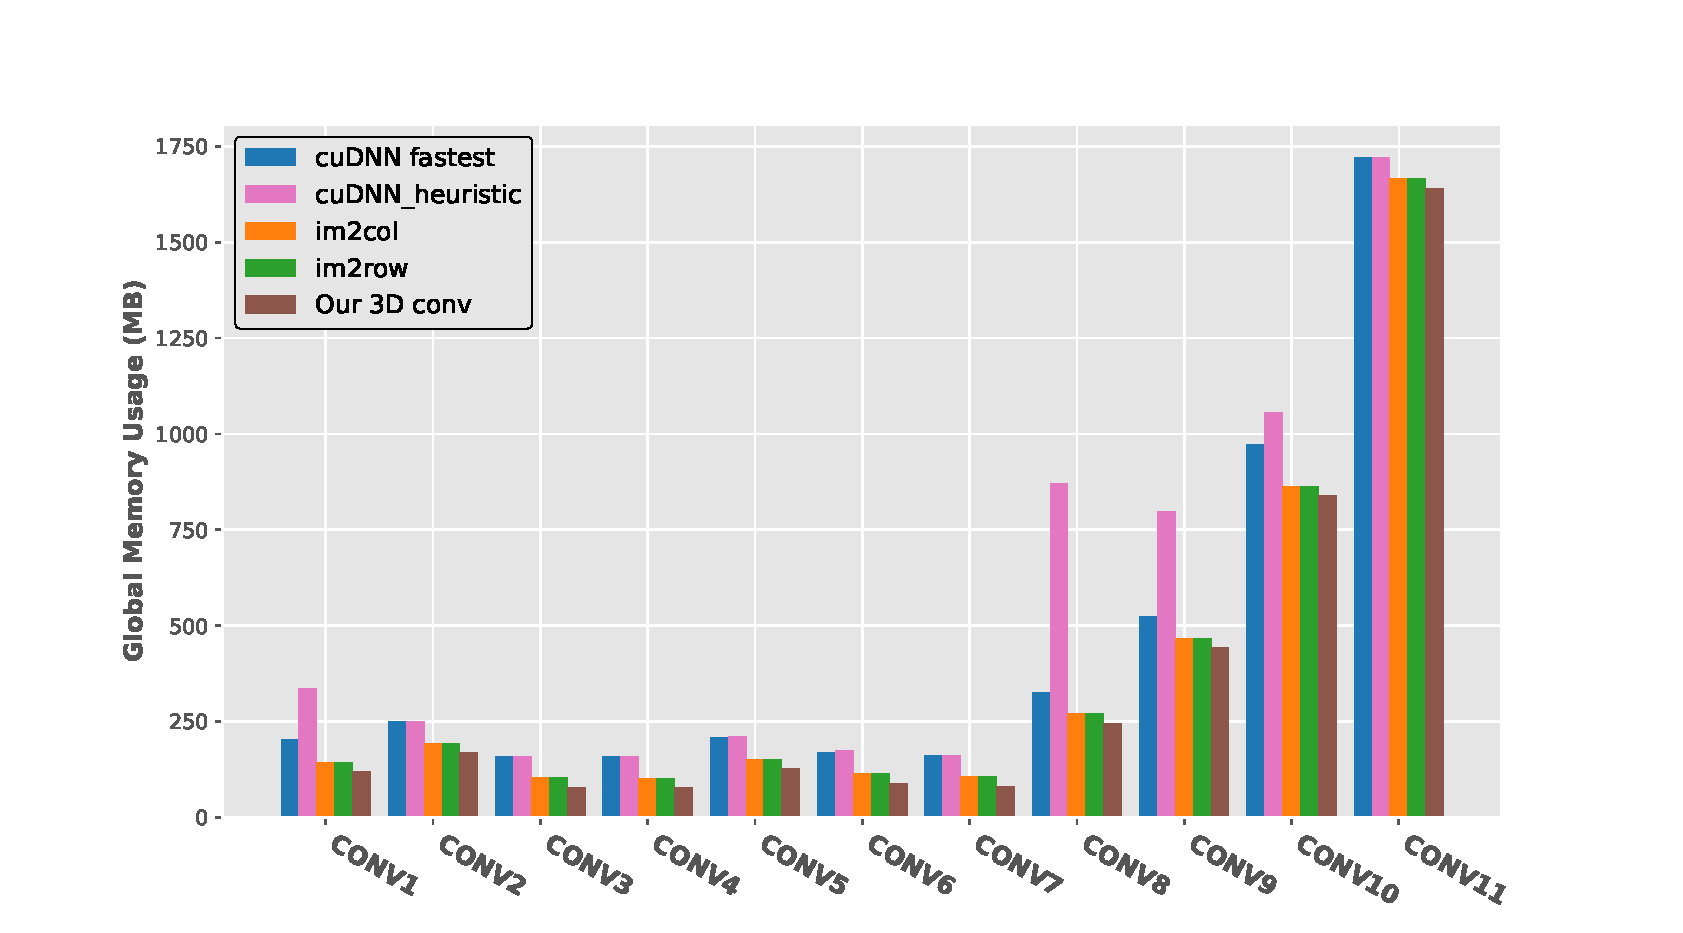
\includegraphics[width=\columnwidth,height=6cm]{./figure/mem3d_1.eps}
%	\label{fig:3dmemk40m}}
%\hspace{0em}
%\subfloat[]{\includegraphics[width=\columnwidth,height=6cm]{./figure/mem3d_1_rtx2080.eps}
%	\label{fig:3dmemrtx2080}}
%
%\caption{Global memory usage for five implementations. Left figure demonstrates the result on Tesla K40m and right figure demonstrates the result on RTX 2080 Ti.}
%\label{fig:3dmem}
%\end{figure*}

We collect configurations of the convolutional layers using depth-wise convolution from three popular mobile CNN models,
namely, MobileNetv2, ShuffleNetv2 and EfficientNet.
Then, we set the number of the batch size to 512 ($I_N=O_N=512$). Other batch sizes demonstrate a similar performance because all tested implementations have a linear scale as the batch size. The exact configuration is presented in Table \ref{tab:3dconvconfigs}.

The speedups are shown in Figure \ref{fig:3druntime}. It is obvious that our implementation performs best in all test cases. We obtain an average speedup of $4.5\times$ and $7.6\times$ for the $3 \times 3$ and $5 \times 5$ filters, respectively. The implicit algorithm is the fastest algorithm in cuDNN in all test cases. It achieves an average speedup of $2.8\times$ and $1.8\times$ for the $3 \times 3$ and $5 \times 5$ filters, respectively. Compared with the fastest algorithm of cuDNN, the proposed approach achieves an average speedup of $1.5\times$, with the maximum speedup reaching $2\times$ for the $3 \times 3$ filter, and an average speedup of $4\times$, with the maximum speedup reaching $4.5\times$ for the $5 \times 5$ filter.

The algorithms of cuDNN except implicit algorithm perform poorly in all test cases and the speedups of these algorithms all below 1. Considering that cuDNN is a closed source, we can only guess that FFT- and Winograd- based algorithms focus on reduction of computation and trades memory performance for speed. Precomp and gemm algorithms need extra memory operations to compute output elements. Moreover, depth-wise convolution is more sensitive to memory performance than multi-channel 2D convolution. Consequently, these algorithms perform poorly on depth-wise convolutions.
 
\begin{figure}
\centering

\subfloat[Memory throughput for the filter of size $3 \times 3$.]{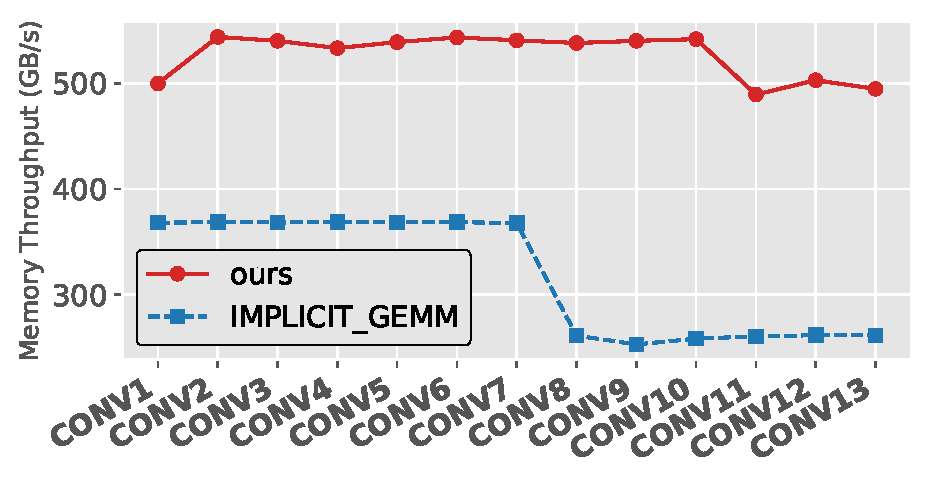
\includegraphics[width=\columnwidth,height=6cm]{./figure/depwisememthroughput.eps}
	\label{fig:depwisememthr}}
\hspace{0em}
\subfloat[Max bandwidth for the filter of size $3 \times 3$.]{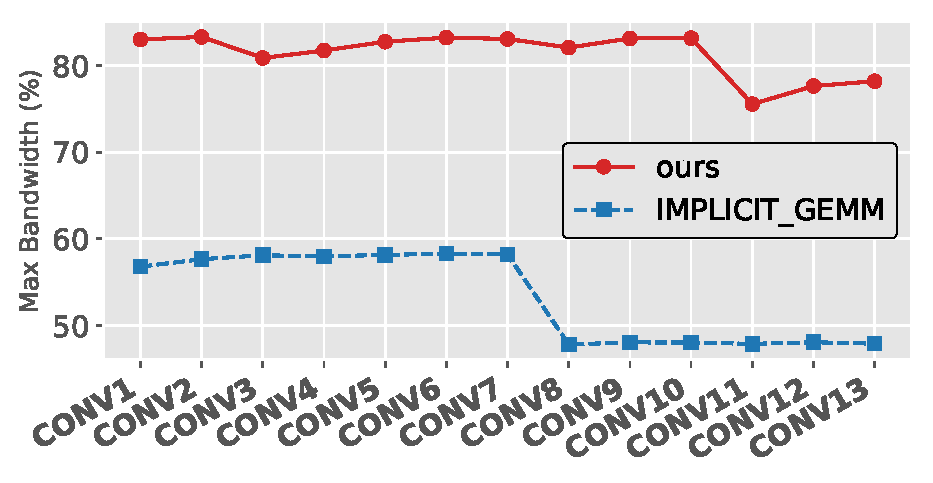
\includegraphics[width=\columnwidth,height=6cm]{./figure/depwisemembandwidth.eps}
	\label{fig:depwisemaxband}}
	
\caption{Memory analysis of cuDNN implicit algorithm and our implementation for the filter of size $3 \times 3$.}
\label{fig:depwisememanaly}
\end{figure}

Figure \ref{fig:depwisememanaly} demonstrates the memory throughput and max bandwidth for our implementation and cuDNN implicit algorithm when convolving with a $3 \times 3$ filter. We can see that our implementation achieves $1.5 times$ memory throughput and max bandwidth compared with the implicit algorithm. This demonstrates that our reuse algorithms can improve the memory performance significantly.
%In contrast to 2D convolutions, the performance gains of 3D convolutions are obtained from two aspects: reduction of the memory transactions of the input data and filters. After loading a filter into the shared memory, we use it to slide over as many images as possible to eliminate the need to load the same filter for each input. Table \ref{tab:3dtrans} lists the number of memory transactions in the four implementations on Tesla K40m. We use the same method used in the 2D convolution to collect the number of memory transactions. Our approach achieves the minimum transaction counts in all tested cases and can reduce the number of memory transactions by a factor of 6.1 and 4.4
%with respect to \emph{cuDNN fastest} with one and three input channels, respectively. Compared with the transaction counts in 2D convolution (Table \ref{tab:2dmemtrans}), that in the 3D convolution has a lower ratio than the other implementations. This phenomenon occurs because in 3D convolutions, each filter needs to slide over all inputs. Hence, we need to load the same filter multiple times. Although we have optimized the use of filters, we still need to load the filters multiple times because the capacity of the shared memory cannot fit the entire
%filters. Consequently, the number of memory transactions increases.

%For 3D convolutions, memory usage is important for the scarce memory storage in GPU. We use \emph{nvidia-smi} command to record the peak GPU device memory usage when the application is running. In this study, we only report the global memory usage for the
%convolutions with one input channel because output data consumes the most memory storage compared with the input and filter data. In addition, changing the number of input channels alone does not change the size of the output data. Therefore, memory usage exhibits only a slight change when we change the number of input channels.

%Figure \ref{fig:3dmem} illustrates the memory usage of the four implementations on two platforms. Our implementation is derived from direct convolution, which does not require extra memory, and therefore consumes the minimum memory storage. GEMM-based implementations (im2col and im2row) first transform the filters into a large matrix before transforming one input into a matrix when performing a matrix multiplication. Therefore, such implementations only need extra memory to store the transformed filters and the transformed input. The most memory consuming
%implementation is cuDNN. Considering that cuDNN is a closed source, we can only guess that this approach improves the performance at the expense of memory usage. The
%memory consumption of our implementation is reduced by 335 MB on average, with the maximum reduction reaching 384 MB with respect to cuDNN fastest. The commonly used
%cuDNN heuristic consumes even more memory than cuDNN fastest. Compared with the cuDNN heuristic, our implementation reduces  memory consumption by 442 MB on average, with the maximum reduction reaching up to 876 MB.

In summary, Both reuse algorithms can significantly improve the memory throughput and max bandwidth, which leads to the improvement of the performance of depth-wise convolutions.  In contrast to cuDNN, which is the state-of-the-art convolution library, our implementation achieves an average speedup of $1.5\times$ and $4\times$ for the $3 \times 3$ and $5 \times 5$ filters, respectively.


\section{Related Work}
Over the past few years, many efforts have been made on optimizing convolution operations. Nowadays, GEMM-based, FFT-based and
Winograd-based convolutions are broadly adopted convolution algorithms.

GEMM-based convolution is the first attempt to optimize convolution. Chellapilla et al. \cite{Chellapilla2006High} developed an unrolling
convolution algorithm which is also called im2col convolution algorithm. They lower the convolutions into a matrix multiplication which is
highly optimized on GPU. Though there are some duplicate input elements involved in the computation, the performance gain is still
impressive. Chetlur et al. \cite{ChetlurWVCTCS14} at NVIDIA integrated the unrolling convolution algorithm into cuDNN.

As general matrix multiplication has been well optimized, researchers shift the focus from GEMM-based convolution to FFT-based and
Winograd-based convolutions. Both FFT-based and Winograd-based convolutions can reduce the computational complexity and improve the
performance of convolution. Mathieu et al. \cite{mathieu2013fast} proposed FFT-based convolution, they compute convolutions as pointwise
products in the Fourier domain and reusing transformed input data many times which significantly reduce the complexity of convolution. This
method greatly improves the performance of convolution compared with GEMM-based implementation. However, FFT-based convolution is more
suitable for large filters, because they need to pad filters to the same size as input data and small filters like $3 \times 3$ need more
memory than large filters. To overcome this drawback, Lavin et al. \cite{lavin2016fast} used Winograd’s minimal filtering algorithm to
accelerate convolution on GPU. Their algorithm can reduce the arithmetic complexity of convolution by up to a factor of 4 compared with
direct convolution. But Winograd algorithm is suitable for small filters due to its numerical instability. \cite{Zhen2018Optimizing}
extends Winograd algorithm to any filter sizes. However, both Winograd-based algorithms need to transform the input and filter before
performing matrix multiplication, and need more operations than FFT algorithm.

All abovementioned convolutions need to transform the input and filter before performing matrix multiplication, this will incur much memory
overhead and offset some performance gains brought by the reduction in computational complexity. Recent studies mainly focus on how to
reduce the memory overhead of transformation phases. \cite{cho2017mec} reduces the memory overhead of GEMM-based convolution. They use a
compact lowering scheme to reduce the redundancy in the lowered matrix and then do multiple small matrix multiplications in parallel.
However, their algorithm still needs to transform the input and filter tensors into lowered matrixes to compute convolution.
\cite{Iandola2014Communication} reduces memory  communication of 2D convolution on GPU. They prefetch image regions to registers, and let
each  thread do more work with fewer threads. Their method just uses registers to accelerate convolution and does not reduce the number of
memory accesses. Different from \cite{Iandola2014Communication}, we further optimize the usage of registers and significantly reduce the
number of memory accesses.

\section{Conclusion}
We have presented two novel approaches to optimize the memory performance and SM utilization for depthwise and pointwise convolutions respectively. 
Our approach improves the data locality for convolutional operations performed on the row and column directions to reduce the memory access. 
Our techniques utilize the common GPU shuffle operations supported by mainstream GPU programming models, including CUDA and OpenCL, and do not require hardware modifications.
For pointwise convolution, the main problem is low SM utilization because cuDNN uses a fixed block strategy for all pointwise convolutions. We design a dynamic block strategy and meanwhile hide the memory access latency. 
We evaluate our approach on an NVIDIA RTX 2080Ti GPU platform. 
We compare our approach against a wide range of heavily optimized convolution algorithms. 
Experimental results show that our approach consistently outperforms the competing methods by delivering the best overall performance for the three types of
convolution tasks.


%For the 2D convolution, our approach outperforms the state-of-the-art image processing libraries. For the depth-wise convolution, our
%techniques deliver up to $4 \times$ speedups over the fastest algorithm of cuDNN. For the multi-channel 2D convolution, proposed reuse
%algorithms achieve an average speedup of $1.23\times$ over the fastest algorithm of cuDNN.


%\begin{acks}                            %% acks environment is optional
%                                        %% contents suppressed with 'anonymous'
%  %% Commands \grantsponsor{<sponsorID>}{<name>}{<url>} and
%  %% \grantnum[<url>]{<sponsorID>}{<number>} should be used to
%  %% acknowledge financial support and will be used by metadata
%  %% extraction tools.
%  This material is based upon work supported by the
%  \grantsponsor{GS100000001}{National Science
%    Foundation}{http://dx.doi.org/10.13039/100000001} under Grant
%  No.~\grantnum{GS100000001}{nnnnnnn} and Grant
%  No.~\grantnum{GS100000001}{mmmmmmm}.  Any opinions, findings, and
%  conclusions or recommendations expressed in this material are those
%  of the author and do not necessarily reflect the views of the
%  National Science Foundation.
%\end{acks}


\section*{Acknowledgments}
This work was supported in part by the National Key Research and Development Program of China under grant agreement 2017YFB0202901, the
Key-Area Research and Development Program of Guangdong Province under grant agreement 2019B010136001, the National Natural Science
Foundation of China (NSFC) under grant agreements 61672186 and 61872294, and the Shenzhen Technology Research and Development Fund under
grant agreement JCYJ20190806143418198. Professor Zhang is the corresponding author.

% Bibliography
\bibliographystyle{IEEEtran}
\bibliography{IEEEabrv,ref}
\begin{IEEEbiography}[{
\includegraphics[width=1in,height=1.25in,clip,keepaspectratio]{figure/GangzhaoLu.eps}}]{Gangzhao Lu}
 received the B.S. degree in computer science and engineering from Harbin Institute of Technology, China, in 2014. He is currently working toward the Ph.D. degree in the School of Cyberspace Science, Harbin Institute of Technology. His research interests include performance modeling, parallel optimization, auto-tuning.
\end{IEEEbiography}
\begin{IEEEbiography}[{
\includegraphics[width=1in,height=1.25in,clip,keepaspectratio]{figure/WeizheZhang.eps}}]{Weizhe Zhang} (Senior Member, IEEE) received B.Eng, M.Eng and Ph.D. degree of Engineering in computer science and technology in 1999, 2001 and 2006 respectively from Harbin Institute of Technology.

He is currently a professor in the School of Computer Science and Technology at Harbin Institute of Technology, China, and director in the Cyberspace Security Research Center, Peng Cheng Laboratory, Shenzhen, China. His research interests are primarily in parallel computing, distributed computing, cloud and grid computing, and computer network. He has published more than 100 academic papers in journals, books, and conference proceedings.
\end{IEEEbiography}
\begin{IEEEbiography}[{
\includegraphics[width=1in,height=1.25in,clip,keepaspectratio]{figure/ZhengWang.eps}}]{Zheng Wang} is
an associate professor with the University of Leeds. His research focuses on parallel computing, compilation and systems security.
\end{IEEEbiography}
\end{document}
